\documentclass[11pt]{article}
\usepackage{units}
\usepackage[small, bf]{caption}
\usepackage[numbers,sort&compress]{natbib}
\usepackage{color}
\usepackage{amssymb, amsmath}
\usepackage{graphicx}
\usepackage{epstopdf}
\usepackage{verbatim}
\usepackage{amsfonts}
\usepackage{subfloat}
\usepackage{subfig}
\usepackage{multirow}
\usepackage{authblk}
\usepackage{array}
\usepackage{footmisc}
\usepackage{tabularx}
\usepackage{sidecap}
\usepackage{setspace}
\usepackage[normalem]{ulem}
\usepackage{pgfplotstable}
\usepackage[margin=1in]{geometry}
\renewcommand\Affilfont{\small}
\newcommand{\ignore}[1]{}
\usepackage{float}

\newenvironment{packed_enum}{
\begin{enumerate}
  \setlength{\itemsep}{1pt}
  \setlength{\parskip}{0pt}
  \setlength{\parsep}{0pt}
}{\end{enumerate}}
\newenvironment{packed_itemize}{
\begin{itemize}
  \setlength{\itemsep}{1pt}
  \setlength{\parskip}{0pt}
  \setlength{\parsep}{0pt}
}{\end{itemize}}
\newenvironment{packed_desc}{
\begin{description}
  \setlength{\itemsep}{1pt}
  \setlength{\parskip}{0pt}
  \setlength{\parsep}{0pt}
}{\end{description}}

\def\AI#1{{\textcolor{red}{#1}}}
\def\dHAF{\text{-HAF}}
\def\HAF{\text{HAF}}
\def\HAFpeak{\text{HAF-peak}}
\def\HAFtrough{\text{HAF-trough}}
\def\HAFneutral{\text{HAF}_{\text{neutral}}}
\def\TMRCA{T_{\text{MRCA}}}

\def\VB#1{{\textcolor{blue}{VB note: #1}}}

\newcommand{\algoname}{\ensuremath{\text{PreCIOSS}}}
\def\vecbold#1{{\boldsymbol#1}}

%%%%%%%%%%%%
\makeatletter
\renewcommand\section{\@startsection {section}{1}{\z@}%                                                                                                         
                                   {-3.2ex \@plus -1ex \@minus -.2ex}%                                                                                        
                                   {2.0ex \@plus.2ex}%                                                                                                        
                                   {\normalfont\Large\bfseries}}
\renewcommand\subsection{\@startsection{subsection}{2}{\z@}%                                                                                                    
                                     {-2.95ex\@plus -1ex \@minus -.2ex}%                                                                                      
                                     {1.2ex \@plus .2ex}%                                                                                                     
                                     {\normalfont\large\bfseries}}
\renewcommand\subsubsection{\@startsection{subsubsection}{3}{\z@}%                                                                                              
                                     {-2.95ex\@plus -1ex \@minus -.2ex}%                                                                                      
                                     {1.2ex \@plus .2ex}%                                                                                                     
                                     {\normalfont\normalsize\bfseries}}
\renewcommand\paragraph{\@startsection{paragraph}{4}{\z@}%                                                                                                      
                                    {1.55ex \@plus1ex \@minus.2ex}%                                                                                           
                                    {-.7em}%                                                                                                                   
                                    {\normalfont\normalsize\bfseries}}
\makeatother
%%%%%%%%%%%%%%%%% Arya's
\usepackage{color,hyperref}
\hypersetup{colorlinks,breaklinks,linkcolor=darkblue,urlcolor=darkblue, anchorcolor=darkblue,citecolor=darkblue}
\usepackage{amssymb,amsmath,amsthm,amsfonts}
\usepackage{mathtools}
\usepackage{enumerate}
\definecolor{darkgreen}{rgb}{0,0.55,0}
\definecolor{orange}{rgb}{1,0.55,0}
\definecolor{darkblue}{rgb}{0.0,0.0,0.5}
\def\Arya#1{{\textcolor{darkgreen}{Arya note: #1}}}
\def\emphr#1{{\textcolor{red}{#1}}}
\def\emphg#1{{\textcolor{darkgreen}{#1}}}
\def\emphb#1{{\textcolor{darkblue}{#1}}}
\usepackage{pifont}
\newcommand{\cmark}{\ding{51}}%
\newcommand{\xmark}{\ding{55}}%
\usepackage{bbm}
\def\datadm{data from a study of \dmel adaptation to alternating temperatures}
\def\comale{\text{{\sc Clear}}}
\newcommand{\dataset}{{\cal D}}
\newcommand{\fracpartial}[2]{\frac{\partial #1}{\partial  #2}}
\newcommand{\phibp}{\phi_{ \hspace{-0.025in}\scalebox{.45}{\text{ BP}}}}
\newcommand{\phics}{\phi_{ \hspace{-0.025in}\scalebox{.45}{\text{ CS}}}}
\newcommand{\lone}{$\ell_1$-norm }
%\def\lll{\mbox{\ell_1}}
\def\dmel{\emph{D. melanogaster }}

\DeclareMathOperator{\tw}{tw}
\DeclareMathOperator{\local}{local}
\DeclareMathOperator{\range}{range}
\DeclareMathOperator{\Path}{Path}
\DeclareMathOperator{\Sg}{Sg}
\DeclareMathOperator{\spt}{SP}
\DeclareMathOperator{\avg}{avg}
\DeclareMathOperator{\nbd}{\mathcal{N}}
\DeclareMathOperator{\parent}{Pa}
\DeclareMathOperator{\Cq}{Cq}
\DeclareMathOperator{\TW}{TW}
\DeclareMathOperator{\approxML}{ApproxML}
\DeclareMathOperator{\Bethe}{Bethe}
\DeclareMathOperator{\TRW}{TRW}
\DeclareMathOperator{\conv}{Conv}
\DeclareMathOperator{\dir}{Dir}
\DeclareMathOperator{\mult}{Mult}
\DeclareMathOperator{\cat}{Cat}
\DeclareMathOperator{\crp}{CRP(\gamma)}
\DeclareMathOperator{\ncrp}{nCRP}
\DeclareMathOperator{\node}{node}
\DeclareMathOperator{\nodes}{nodes}
\DeclareMathOperator{\pr}{Pr}
\DeclareMathOperator{\dom}{\bf Dom}
\DeclareMathOperator{\lbp}{LBP}
\DeclareMathOperator{\Corr}{Corr}
\DeclareMathOperator{\hCorr}{\widehat{Corr}}
\DeclareMathOperator{\hSc}{\widehat{\mathcal{S}}}
\DeclareMathOperator{\tr}{Tr}
\DeclareMathOperator{\mst}{MST}
\DeclareMathOperator{\supp}{Supp}
\DeclareMathOperator{\dtv}{d_{TV}}
\DeclareMathOperator{\hdtv}{\hd_{TV}}
\DeclareMathOperator*{\argmin}{arg\,min}
\DeclareMathOperator*{\argmax}{arg\,max}
\DeclareMathOperator*{\esssup}{ess\,sup}
\DeclareMathOperator*{\essinf}{ess\,inf}
\DeclareMathOperator{\dist}{dist}
\DeclareMathOperator{\rank}{Rank}
\DeclareMathOperator{\Krank}{Rank_K}
\DeclareMathOperator{\Det}{Det}
\DeclareMathOperator{\poiss}{Poiss}
\DeclareMathOperator{\unif}{Unif} \DeclareMathOperator{\Deg}{Deg}
\def\simiid{{\overset{i.i.d.}{\sim}}}
\def\lcv{{\,\,\underset{cv}{\leq}\,\,}}
\def\gcv{{\,\,\underset{cv}{\geq}\,\,}}
\def\lcx{{\,\,\underset{cx}{\leq}\,\,}}
\def\gcx{{\,\,\underset{cx}{\geq}\,\,}}
\def\leqst{{\,\,\overset{st}{\leq}\,\,}}
\def\geqst{{\,\,\overset{st}{\geq}\,\,}}
\def\eqdist{{\,\,\overset{d}{=}\,\,}}
\def\geqrh{{\,\,\overset{rh}{\geq}\,\,}}
\def\geqlr{{\,\,\overset{lr}{\geq}\,\,}}
\def\eqlr{{\,\,\overset{lr}{=}\,\,}}
\def\tha{{\mbox{\tiny th}}}

\DeclareMathOperator{\Aug}{Aug}
\DeclareMathOperator{\watts}{Watts}
\DeclareMathOperator{\girth}{Girth}
\DeclareMathOperator{\PL}{PL}
\DeclareMathOperator{\LP}{LP}
\DeclareMathOperator{\ER}{ER}
\DeclareMathOperator{\reg}{Reg}
\DeclareMathOperator{\Var}{Var}
\DeclareMathOperator{\hSigma}{\widehat{\Sigma}}
\DeclareMathOperator{\Cov}{Cov}
\DeclareMathOperator{\Poiss}{Poiss}
\DeclareMathOperator{\Diag}{Diag}
\DeclareMathOperator{\Diam}{Diam}
\def\erf{\mbox{erf}}
\def\erfc{\mbox{erfc}}
\def\qfunc{\mbox{Q}}
%\def\myexp{\mbox{e}}
\def\snr{\mbox{{SNR}}}
\def\signum{\mbox{sgn}}
\def\Card{\mbox{Card}}
\DeclareMathOperator*{\plim}{plim}
\def\convd{\overset{d}\rightarrow}
\def\convp{\overset{p}\rightarrow}
\newcommand\indep{\protect\mathpalette{\protect\independenT}{\perp}}
\def\independenT#1#2{\mathrel{\rlap{$#1#2$}\mkern2mu{#1#2}}}
\def\pl{{\parallel}}
\DeclarePairedDelimiter\norm{\lVert}{\rVert}
\DeclarePairedDelimiter\nuclearnorm{\lVert}{\rVert_*}
\DeclarePairedDelimiter\onenorm{\lVert}{\rVert_1}
\DeclarePairedDelimiter\znorm{\lVert}{\rVert_0}
\def\rinfnorm{\rVert_{\infty}}
\DeclarePairedDelimiter\infnorm{\lVert}{\rinfnorm}
\def\lnorm{{\lvert\!\lvert\!\lvert}}
\def\rnorm{{\rvert\!\rvert\!\rvert}}
\DeclarePairedDelimiter\gennorm{\lnorm}{\rnorm}
 \DeclarePairedDelimiter\abs{\lvert}{\rvert}
 \DeclarePairedDelimiter\geninfnorm{\lnorm}{\rnorm_{\infty}}
 \DeclarePairedDelimiter\genonenorm{\lnorm}{\rnorm_{1}}
\DeclareMathOperator{\atanh}{atanh}
 \DeclareMathOperator{\sech}{sech}
 \def\0{{\bf 0}}

\DeclareMathOperator{\lea}{\overset{(a)}{\leq}}
\DeclareMathOperator{\leb}{\overset{(b)}{\leq}}
\DeclareMathOperator{\lec}{\overset{(c)}{\leq}}
\DeclareMathOperator{\led}{\overset{(d)}{\leq}}
\DeclareMathOperator{\lee}{\overset{(e)}{\leq}}

\DeclareMathOperator{\eqa}{\overset{(a)}{=}}
\DeclareMathOperator{\eqb}{\overset{(b)}{=}}
\DeclareMathOperator{\eqc}{\overset{(c)}{=}}
\DeclareMathOperator{\eqd}{\overset{(d)}{=}}
\DeclareMathOperator{\eqe}{\overset{(e)}{=}}

\DeclareMathOperator{\gea}{\overset{(a)}{\geq}}
\DeclareMathOperator{\geb}{\overset{(b)}{\geq}}
\DeclareMathOperator{\gec}{\overset{(c)}{\geq}}
\DeclareMathOperator{\ged}{\overset{(d)}{\geq}}
\DeclareMathOperator{\gee}{\overset{(e)}{\geq}}

\def\viz{{viz.,\ \/}}
\def\ie{{i.e.,\ \/}}
\def\eg{{e.g.,\ \/}}
\def\etc{{etc.  }}
\def\ifff{{iff  }}
\def\as{{a.s.  }}
\def\st{{s.t.  }}
\def\wpone{{w.p.}\,1\,\,}
\def\wpp{{w.p.p.}\,\,}
\def\for{\,\,\mbox{for}\quad}
\def\ifmbox{\,\,\mbox{if}\quad}
\def\nn{\nonumber}
%\def\qed{\hfill$\Box$}

\def\qed{\hfill\hbox{${\vcenter{\vbox{
    \hrule height 0.4pt\hbox{\vrule width 0.4pt height 6pt
    \kern5pt\vrule width 0.4pt}\hrule height 0.4pt}}}$}}
\def\complx{\mathbb{C}}

%%%%%%%%%%%%%%%%%%%%%%%%%%%%%%%%%%%%%%%%%%%%%%%%%%%%%%%%%%%%% Color

\def\tcr{\textcolor{red}}
\def\tcb{\textcolor{blue}}
\def\tcg{\textcolor{green}}
\def\tcw{\textcolor{white}}
\def\tcm{\textcolor{magenta}}
\def\tccyan{\textcolor{cyan}}
\def\tcv{\textcolor{violet}}
\definecolor{myred}{rgb}{0.3,0.0,0.7}
\definecolor{dkg}{rgb}{0.1,0.7,0.2}
\definecolor{dkb}{rgb}{0.0,0.2,0.8}

\def\tcdkb{\textcolor{dkb}}
\def\tcdkg{\textcolor{dkg}}


%%%%%%%%%%%%%%%%%%%%%%%%%%%%%%%%%%%%%%%%%%%%%%%%%%%%%%%%%%%%%
\newcommand{\Amsc}{\mathscr{A}}
\newcommand{\Cmsc}{\mathscr{C}}
\newcommand{\Dmsc}{\mathscr{D}}
\newcommand{\Emsc}{\mathscr{E}}
\newcommand{\Fmsc}{\mathscr{F}}
\newcommand{\Gmsc}{\mathscr{G}}
\newcommand{\Hmsc}{\mathscr{H}}
\newcommand{\Kmsc}{\mathscr{K}}
\newcommand{\Nmsc}{\mathscr{N}}
\newcommand{\Pmsc}{\mathscr{P}}
\newcommand{\Qmsc}{\mathscr{Q}}
\newcommand{\Rmsc}{\mathscr{R}}
\newcommand{\Smsc}{\mathscr{S}}
\newcommand{\Tmsc}{\mathscr{T}}
\newcommand{\Umsc}{\mathscr{U}}
\newcommand{\Xmsc}{\mathscr{X}}
\newcommand{\Ymsc}{\mathscr{Y}}

%%%%%%%%%%%%%%%%%%%%%%%%%%%%%%%%%%%%%%%%%%%%%%%%%%%%%%%%%%%%% Hat
\def\ha{\widehat{a}}
\def\hb{\widehat{b}}
\def\hc{\widehat{c}}
\def\hd{\widehat{d}}
\def\he{\widehat{e}}
\def\hf{\widehat{f}}
\def\hg{\widehat{g}}
\def\hh{\widehat{h}}
\def\hi{\widehat{i}}
\def\hj{\widehat{j}}
\def\hk{\widehat{k}}
\def\hl{\widehat{l}}
\def\hm{\widehat{m}}
\def\hn{\widehat{n}}
\def\ho{\widehat{o}}
\def\hp{\widehat{p}}
\def\hq{\widehat{q}}
\def\hr{\widehat{r}}
\def\hs{\widehat{s}}
\def\hatt{\widehat{t}}
\def\hu{\widehat{u}}
\def\hv{\widehat{v}}
\def\hw{\widehat{w}}
\def\hx{\widehat{x}}
\def\hy{\widehat{y}}
\def\hz{\widehat{z}}

\def\hA{\widehat{A}}
\def\hB{\widehat{B}}
\def\hC{\widehat{C}}
\def\hD{\widehat{D}}
\def\hE{\widehat{E}}
\def\hF{\widehat{F}}
\def\hG{\widehat{G}}
\def\hH{\widehat{H}}
\def\hI{\widehat{I}}
\def\hJ{\widehat{J}}
\def\hK{\widehat{K}}
\def\hL{\widehat{L}}
\def\hM{\widehat{M}}
\def\hN{\widehat{N}}
\def\hO{\widehat{O}}
\def\hP{\widehat{P}}
\def\hQ{\widehat{Q}}
\def\hR{\widehat{R}}
\def\hS{\widehat{S}}
\def\hT{\widehat{T}}
\def\hU{\widehat{U}}
\def\hV{\widehat{V}}
\def\hW{\widehat{W}}
\def\hX{\widehat{X}}
\def\hY{\widehat{Y}}
\def\hZ{\widehat{Z}}
\def\hlambda{\widehat{\lambda}}
\def\hpi{\widehat{\pi}}
\def\hnu{\widehat{\nu}}
\def\hbd{\widehat{\mathbf{d}}}
\def\bLambda{\mathbf{\Lambda}}


%%%%%%%%%%%%%%%%%%%%%%%%%%%%%%%%%%%%%%%%%%%%%%%%%%%%%%%%%%%%% Vector
\def\valpha{\vec{\alpha}}
\def\va{\vec{a}}
\def\vb{\vec{b}}
\def\vc{\vec{c}}
\def\vd{\vec{d}}
\def\ve{\vec{e}}
\def\vf{\vec{f}}
\def\vg{\vec{g}}
\def\vh{\vec{h}}
\def\vi{\vec{i}}
\def\vj{\vec{j}}
\def\vk{\vec{k}}
\def\vl{\vec{l}}
\def\vm{\vec{m}}
\def\vn{\vec{n}}
\def\vo{\vec{o}}
\def\vp{\vec{p}}
\def\vq{\vec{q}}
\def\vr{\vec{r}}
\def\vs{\vec{s}}
\def\vt{\vec{t}}
\def\vu{\vec{u}}
\def\vv{\vec{v}}
\def\vw{\vec{w}}
\def\vx{\vec{x}}
\def\vy{\vec{y}}
\def\vz{\vec{z}}

\def\vA{\vec{A}}
\def\vB{\vec{B}}
\def\vC{\vec{C}}
\def\vD{\vec{D}}
\def\vE{\vec{E}}
\def\vF{\vec{F}}
\def\vG{\vec{G}}
\def\vH{\vec{H}}
\def\vI{\vec{I}}
\def\vJ{\vec{J}}
\def\vK{\vec{K}}
\def\vL{\vec{L}}
\def\vM{\vec{M}}
\def\vN{\vec{N}}
\def\vO{\vec{O}}
\def\vP{\vec{P}}
\def\vQ{\vec{Q}}
\def\vR{\vec{R}}
\def\vS{\vec{S}}
\def\vT{\vec{T}}
\def\vU{\vec{U}}
\def\vV{\vec{V}}
\def\vW{\vec{W}}
\def\vX{\vec{X}}
\def\vY{\vec{Y}}
\def\vZ{\vec{Z}}

%%%%%%%%%%%%%%%%%%%%%%%%%%%%%%%%%%%%%%%%%%%%%%%%%%%%%%%%%%%%% Bold
\def\bfalpha{{\boldsymbol {\alpha}}}
\def\bfnu{{\boldsymbol {\nu}}}
\def\bfeta{{\boldsymbol {\eta}}}
\def\bfzero{{\mathbf{0}}}
\def\bfone{{\mathbf{1}}}
\def\bfa{{\mathbf a}}
\def\bfb{{\mathbf b}}
\def\bfc{{\mathbf c}}
\def\bfd{{\mathbf d}}
\def\bfe{{\mathbf e}}
\def\bff{{\mathbf f}}
\def\bfg{{\mathbf g}}
\def\bfh{{\mathbf h}}
\def\bfi{{\mathbf i}}
\def\bfj{{\mathbf j}}
\def\bfk{{\mathbf k}}
\def\bfl{{\mathbf l}}
\def\bfm{{\mathbf m}}
\def\bfn{{\mathbf n}}
\def\bfo{{\mathbf o}}
\def\bfp{{\mathbf p}}
\def\bfq{{\mathbf q}}
\def\bfr{{\mathbf r}}
\def\bfs{{\mathbf s}}
\def\bft{{\mathbf t}}
\def\bfu{{\mathbf u}}
\def\bfv{{\mathbf v}}
\def\bfw{{\mathbf w}}
\def\bfx{{\mathbf x}}
\def\bfy{{\mathbf y}}
\def\bfz{{\mathbf z}}

\def\bfA{{\mathbf A}}
\def\bfB{{\mathbf B}}
\def\bfC{{\mathbf C}}
\def\bfD{{\mathbf D}}
\def\bfE{{\mathbf E}}
\def\bfF{{\mathbf F}}
\def\bfG{{\mathbf G}}
\def\bfH{{\mathbf H}}
\def\bfI{{\mathbf I}}
\def\bfJ{{\mathbf J}}
\def\bfK{{\mathbf K}}
\def\bfL{{\mathbf L}}
\def\bfM{{\mathbf M}}
\def\bfN{{\mathbf N}}
\def\bfO{{\mathbf O}}
\def\bfP{{\mathbf P}}
\def\bfQ{{\mathbf Q}}
\def\bfR{{\mathbf R}}
\def\bfS{{\mathbf S}}
\def\bfT{{\mathbf T}}
\def\bfU{{\mathbf U}}
\def\bfV{{\mathbf V}}
\def\bfW{{\mathbf W}}
\def\bfX{{\mathbf X}}
\def\bfY{{\mathbf Y}}
\def\bfZ{{\mathbf Z}}


%%%%%%%%%%%%%%%%%%%%%%%%%%%%%%%%%%%%%%%%%%%%%%%%%%%%%%%%%%%%% Bold Symbols
\def\alphabf{\hbox{\boldmath$\alpha$\unboldmath}}
\def\betabf{\hbox{\boldmath$\beta$\unboldmath}}
\def\gammabf{\hbox{\boldmath$\gamma$\unboldmath}}
\def\deltabf{\hbox{\boldmath$\delta$\unboldmath}}
\def\epsilonbf{\hbox{\boldmath$\epsilon$\unboldmath}}
\def\zetabf{\hbox{\boldmath$\zeta$\unboldmath}}
\def\etabf{\hbox{\boldmath$\eta$\unboldmath}}
\def\iotabf{\hbox{\boldmath$\iota$\unboldmath}}
\def\kappabf{\hbox{\boldmath$\kappa$\unboldmath}}
\def\lambdabf{\hbox{\boldmath$\lambda$\unboldmath}}
\def\mubf{\hbox{\boldmath$\mu$\unboldmath}}
\def\nubf{\hbox{\boldmath$\nu$\unboldmath}}
\def\xibf{\hbox{\boldmath$\xi$\unboldmath}}
\def\pibf{\hbox{\boldmath$\pi$\unboldmath}}
\def\rhobf{\hbox{\boldmath$\rho$\unboldmath}}
\def\sigmabf{\hbox{\boldmath$\sigma$\unboldmath}}
\def\taubf{\hbox{\boldmath$\tau$\unboldmath}}
\def\upsilonbf{\hbox{\boldmath$\upsilon$\unboldmath}}
\def\phibf{\hbox{\boldmath$\phi$\unboldmath}}
\def\chibf{\hbox{\boldmath$\chi$\unboldmath}}
\def\psibf{\hbox{\boldmath$\psi$\unboldmath}}
\def\omegabf{\hbox{\boldmath$\omega$\unboldmath}}
\def\inftybf{\hbox{\boldmath$\infty$\unboldmath}}
\def\hSigmabf{\hbox{$\widehat{\bf \Sigma}$}}
\def\Sigmabf{\hbox{$\bf \Sigma$}}
\def\Upsilonbf{\hbox{$\bf \Upsilon$}}
\def\Omegabf{\hbox{$\bf \Omega$}}
\def\Deltabf{\hbox{$\bf \Delta$}}
\def\Gammabf{\hbox{$\bf \Gamma$}}
\def\Thetabf{\hbox{$\bf \Theta$}}
\def\Lambdabf{\mbox{$ \bf \Lambda $}}
\def\Xibf{\hbox{\bf$\Xi$}}
\def\Pibf{{\bf \Pi}}
\def\thetabf{{\mbox{\boldmath$\theta$\unboldmath}}}
\def\Upsilonbf{\hbox{\boldmath$\Upsilon$\unboldmath}}
\newcommand{\Phibf}{\mbox{${\bf \Phi}$}}
\newcommand{\Psibf}{\mbox{${\bf \Psi}$}}
\def\olambda{\mathfrak{o}(\lambda)}
\def\complex{\mathfrak{C}}

%%%%%%%%%%%%%%%%%%%%%%%%%%%%%%%%%%%%%%%%%%%%%%%%%%%%%%%%%%%%% Bar
\def\brzero{{\overline{{0}}}}
\def\brone{{\overline{{1}}}}
\def\bra{{\overline{a}}}
\def\brb{{\overline{b}}}
\def\brc{{\overline{c}}}
\def\brd{{\overline{d}}}
\def\bre{{\overline{e}}}
\def\brf{{\overline{f}}}
\def\brg{{\overline{g}}}
\def\brh{{\overline{h}}}
\def\bri{{\overline{i}}}
\def\brj{{\overline{j}}}
\def\brk{{\overline{k}}}
\def\brl{{\overline{l}}}
\def\brm{{\overline{m}}}
\def\brn{{\overline{n}}}
\def\bro{{\overline{o}}}
\def\brp{{\overline{p}}}
\def\brq{{\overline{q}}}
\def\brr{{\overline{r}}}
\def\brs{{\overline{s}}}
\def\brt{{\overline{t}}}
\def\bru{{\overline{u}}}
\def\brv{{\overline{v}}}
\def\brw{{\overline{w}}}
\def\brx{{\overline{x}}}
\def\bry{{\overline{y}}}
\def\brz{{\overline{z}}}

\def\brA{{\overline{A}}}
\def\brB{{\overline{B}}}
\def\brC{{\overline{C}}}
\def\brD{{\overline{D}}}
\def\brE{{\overline{E}}}
\def\brF{{\overline{F}}}
\def\brG{{\overline{G}}}
\def\brH{{\overline{H}}}
\def\brI{{\overline{I}}}
\def\brJ{{\overline{J}}}
\def\brK{{\overline{K}}}
\def\brL{{\overline{L}}}
\def\brM{{\overline{M}}}
\def\brN{{\overline{N}}}
\def\brO{{\overline{O}}}
\def\brP{{\overline{P}}}
\def\brQ{{\overline{Q}}}
\def\brR{{\overline{R}}}
\def\brS{{\overline{S}}}
\def\brT{{\overline{T}}}
\def\brU{{\overline{U}}}
\def\brV{{\overline{V}}}
\def\brW{{\overline{W}}}
\def\brX{{\overline{X}}}
\def\brY{{\overline{Y}}}
\def\beZ{{\overline{Z}}}

%%%%%%%%%%%%%%%%%%%%%%%%%%%%%%%%%%%%%%%%%%%%%%%%%%%%%%%%%%%%% Bar Bold 
\def\bbfzero{{\overline{\mathbf{0}}}}
\def\bbfone{{\overline{\mathbf{1}}}}
\def\bbfa{{\overline{\mathbf a}}}
\def\bbfb{{\overline{\mathbf b}}}
\def\bbfc{{\overline{\mathbf c}}}
\def\bbfd{{\overline{\mathbf d}}}
\def\bbfe{{\overline{\mathbf e}}}
\def\bbff{{\overline{\mathbf f}}}
\def\bbfg{{\overline{\mathbf g}}}
\def\bbfh{{\overline{\mathbf h}}}
\def\bbfi{{\overline{\mathbf i}}}
\def\bbfj{{\overline{\mathbf j}}}
\def\bbfk{{\overline{\mathbf k}}}
\def\bbfl{{\overline{\mathbf l}}}
\def\bbfm{{\overline{\mathbf m}}}
\def\bbfn{{\overline{\mathbf n}}}
\def\bbfo{{\overline{\mathbf o}}}
\def\bbfp{{\overline{\mathbf p}}}
\def\bbfq{{\overline{\mathbf q}}}
\def\bbfr{{\overline{\mathbf r}}}
\def\bbfs{{\overline{\mathbf s}}}
\def\bbft{{\overline{\mathbf t}}}
\def\bbfu{{\overline{\mathbf u}}}
\def\bbfv{{\overline{\mathbf v}}}
\def\bbfw{{\overline{\mathbf w}}}
\def\bbfx{{\overline{\mathbf x}}}
\def\bbfy{{\overline{\mathbf y}}}
\def\bbfz{{\overline{\mathbf z}}}

\def\bbfA{{\overline{\mathbf A}}}
\def\bbfB{{\overline{\mathbf B}}}
\def\bbfC{{\overline{\mathbf{C}}}}
\def\bbfD{{\overline{\mathbf D}}}
\def\bbfE{{\overline{\mathbf E}}}
\def\bbfF{{\overline{\mathbf F}}}
\def\bbfG{{\overline{\mathbf G}}}
\def\bbfH{{\overline{\mathbf H}}}
\def\bbfI{{\overline{\mathbf I}}}
\def\bbfJ{{\overline{\mathbf J}}}
\def\bbfK{{\overline{\mathbf K}}}
\def\bbfL{{\overline{\mathbf L}}}
\def\bbfM{{\overline{\mathbf M}}}
\def\bbfN{{\overline{\mathbf N}}}
\def\bbfO{{\overline{\mathbf O}}}
\def\bbfP{{\overline{\mathbf P}}}
\def\bbfQ{{\overline{\mathbf Q}}}
\def\bbfR{{\overline{\mathbf R}}}
\def\bbfS{{\overline{\mathbf S}}}
\def\bbfT{{\overline{\mathbf T}}}
\def\bbfU{{\overline{\mathbf U}}}
\def\bbfV{{\overline{\mathbf V}}}
\def\bbfW{{\overline{\mathbf W}}}
\def\bbfX{{\overline{\mathbf X}}}
\def\bbfY{{\overline{\mathbf Y}}}
\def\bbfZ{{\overline{\mathbf Z}}}

%%%%%%%%%%%%%%%%%%%%%%%%%%%%%%%%%%%%%%%%%%%%%%%%%%%%%%%%%%%%% Calligraphic
\def\Ac{{\cal A}}
\def\Bc{{\cal B}}
\def\Cc{{\cal C}}
\def\Dc{{\cal D}}
\def\Ec{{\cal E}}
\def\Fc{{\cal F}}
\def\Gc{{\cal G}}
\def\Hc{{\cal H}}
\def\Ic{{\cal I}}
\def\Jc{{\cal J}}
\def\Kc{{\cal K}}
\def\Lc{{\cal L}}
\def\Mc{{\cal M}}
\def\Nc{{\cal N}}
\def\Oc{{\cal O}}
\def\Pc{{\cal P}}
\def\Qc{{\cal Q}}
\def\Rc{{\cal R}}
\def\Sc{{\cal S}}
\def\Tc{{\cal T}}
\def\Uc{{\cal U}}
\def\Vc{{\cal V}}
\def\Wc{{\cal W}}
\def\Xc{{\cal X}}
\def\Yc{{\cal Y}}
\def\Zc{{\cal Z}}


%%%%%%%%%%%%%%%%%%%%%%%%%%%%%%%%%%%%%%%%%%%%%%%%%%%%%%%%%%%%% Mathbb

\def\Abb{{\mathbb A}}
\def\BBb{{\mathbb B}}% different
\def\Cbb{{\mathbb C}}
\def\Dbb{{\mathbb D}}
\def\Ebb{{\mathbb E}}
\def\Fbb{{\mathbb F}}
\def\Gbb{{\mathbb G}}
\def\Hbb{{\mathbb H}}
\def\Ibb{{\mathbb I}}
\def\Jbb{{\mathbb J}}
\def\Kbb{{\mathbb K}}
\def\Lbb{{\mathbb L}}
\def\Mbb{{\mathbb M}}
\def\Nbb{{\mathbb N}}
\def\Obb{{\mathbb O}}
\def\Pbb{{\mathbb P}}
\def\Qbb{{\mathbb Q}}
\def\Rbb{{\mathbb R}}
\def\Sbb{{\mathbb S}}
\def\Tbb{{\mathbb T}}
\def\Ubb{{\mathbb U}}
\def\Vbb{{\mathbb V}}
\def\Wbb{{\mathbb W}}
\def\Xbb{{\mathbb X}}
\def\Ybb{{\mathbb Y}}
\def\Zbb{{\mathbb Z}}
\def\xbb{{\mathbbm x}}

%%%%%%%%%%%%%%%%%%%%%%%%%%%%%%%%%%%%%%%%%%%%%%%%%%%%%%%%%%%%% Command Abbreviations
%\newtheorem{theorem}{Theorem}
%\newtheorem{lemma}{Lemma}
%\newcommand{\bprfof}{\begin{proof_of}}
%\newcommand{\eprfof}{\end{proof_of}}
\newcommand{\bprf}{\begin{proof}}
\newcommand{\eprf}{\end{proof}}
%\newcommand{\bp}{\begin{psfrags}}
%\newcommand{\ep}{\end{psfrags}}
\newcommand{\bl}{\begin{lemma}}
\newcommand{\el}{\end{lemma}}
\newcommand{\bt}{\begin{theorem}}
\newcommand{\et}{\end{theorem}}
%\newcommand{\bc}{\begin{center}}
%\newcommand{\ec}{\end{center}}
%\newcommand{\bi}{\begin{itemize}}
%\newcommand{\ei}{\end{itemize}}
%\newcommand{\ben}{\begin{enumerate}}
%\newcommand{\een}{\end{enumerate}}
%\newcommand{\bd}{\begin{definition}}
%\newcommand{\ed}{\end{definition}}
\def\beq{\begin{equation}\begin{aligned}}
\def\eeq{\end{aligned}\end{equation}\noindent}
\def\beqq{\begin{equation*}\begin{aligned}}
\def\eeqq{\end{aligned}\end{equation*}\noindent}
\def\beqn{\begin{eqnarray}}
\def\eeqn{\end{eqnarray} \noindent}
%\def\beqnn{  \begin{eqnarray*}}
%\def\eeqnn{\end{eqnarray*}  \noindent}
%\def\bcase{  \begin{numcases}}
%\def\ecase{\end{numcases}   \noindent}
%\def\bsbcase{  \begin{subnumcases}}
%\def\esbcase{\end{subnumcases}   \noindent}
%
%\def\endproof{\hfill\blacksquare}
%\def\defeq{{:=}}%{{\stackrel{\Delta}{=}}}
%
%

\title{\comale: Analyzing Adaptive Experimental Evolution with Pooled Sequencing Data}
\author[1]{Arya Iranmehr}
\author[1]{Ali Akbari}
\author[2]{Christian Schl\"{o}tterer}
\author[3]{Vineet Bafna}
\affil[1]{\footnotesize Electrical and Computer Engineering, University of California, San Diego, La Jolla, CA 92093, USA.}
\affil[2]{\footnotesize Institut f\"{u}r Populationsgenetik, Vetmeduni, Vienna, Austria.}
\affil[3]{\footnotesize Computer Science \& Engineering, University of California, San Diego, La Jolla, CA 92093, USA}
\date{}
\def\comale{\text{{\sc Comale}}}
\renewcommand{\figurename}{Fig.}


\begin{document}
\maketitle
\begin{abstract}
  Experimental evolution (EE) studies are powerful tools for observing
  molecular evolution ``in-action'' in populations sampled in
  controlled and natural environments. The advent of sequencing
  technologies has made whole-genome and whole-population sampling
  possible even for eukaryotic organisms with large genomes, and
  allowed us to locate the genes and variants responsible for genetic
  adaptation. While many computational tests have been developed for
  detecting regions under selection, they are mainly designed for
  static (single time) data, and work best when the favored allele is
  close to fixation. 

  EE studies provide samples over multiple time points, underscoring
  the need for tools that can exploit the data. At the same time, EE
  studies are constrained by the limited time span since onset of
  selection, depending upon the generation time for the organism. This
  constraint impedes adaptation and optimization studies, as the
  population can only be propagated for a small number of generations,
  relative to the fixation time of the favored allele.  Moreover,
  sequencing depths of pooled experiments vary across replicates and
  time points, leading to ascertainment bias.

 %In the course of an EE study, multiple replicates of population are
 %sampled and sequenced using pooled-sequencing techniques.  Reads of
 %each locus reads are mapped for all replicates and generations.
 %Even if the sequencing coverage be the same for all the generations
 %and replicates, depth of each site would not necessarily be the
 %same, which leads to the problem of heterogeneous ascertainment bias
 %across generations.

  In this article, we directly address these issues while developing
  tools for identifying selective sweep in short-term and
  pool-sequenced experimental evolution of sexual organisms and
  propose Composite Of MArkovian Likelihoods for Experimental
  evolution (\comale) statistic. Extensive simulations show that
  \comale\ achieves higher detection power over a wide range of
  parameters, including both soft and hard sweep scenarios, and is
  many orders of magnitude faster than other methods, making genomic
  scans feasible.  We apply the \comale\ statistic to the controlled
  experimental evolution of D. melanogaster to detect adaptive
  genes/alleles under alternating cold and hot temperatures, and
  identify many genes that are adapting to the selection constraints.
  \end{abstract}




\section{Introduction}
Natural selection is the key force in evolution, and a mechanism by
which populations can adapt to external `selection'
constraints. Examples of adaptation abound in the natural world,
including for example, classic examples like lactose tolerance in
Northern Europeans~\cite{bersaglieri2004genetic}, human adaptation to high
altitudes~\cite{yi2010sequencing,simonson2010genetic}, but also drug 
resistance in
pests~\cite{daborn2001ddt}, HIV~\cite{Feder2016More},
cancer~\cite{gottesman2002mechanisms,zahreddine2013mechanisms},
malarial parasite~\cite{ariey2014molecular,nair2007recurrent}, and
other antibiotic resistance~\cite{spellberg2008epidemic}. In each of
these examples, understanding the genetic basis of adaptation can
provide actionable information, underscoring the importance of the
problem.

Modern experimental evolution refers to the study of the evolutionary
processes of a model organism at genomic level in a controlled
\cite{hegreness2006equivalence,lang2013pervasive,orozco2012adaptation,
  lang2011genetic,barrick2009genome,bollback2007clonal,oz2014strength}
or natural
\cite{maldarelli2013hiv,reid2011new,denef2012situ,winters2012development,
  daniels2013genetic,barrett2008natural,bergland2014genomic}
environment. Recent advances in whole genome sequencing have enabled
us to sequence populations at a reasonable cost even when the genomes
are large. Perhaps more important for experimental evolution studies,
we can now obtain and sequence \emph{longitudinal time-series data},
sampling populations over a period of time, and investigating the
dynamics of evolution at molecular level.  Although constraints such
as small population sizes, limited timescales, and oversimplified
laboratory environments limit the interpretation of EE results, these
studies are increasingly being used to test hypotheses regarding
mutation rate, inbreeding, environmental variability, sexual selection
\& conflict, kin selection and cooperation, life history and sex
allocation, sexual reproduction and mating systems, behavior and
cognition, and host-–parasite
interactions~\cite{kawecki2012experimental}. In many cases, they
provide more accurate inferences than static data analysis
\cite{boyko2008assessing,desai2008polymorphism,sawyer1992population}. Dynamic
data is also being used to estimate model parameters including
population
size~\cite{williamson1999using,wang2001pseudo,pollak1983new,waples1989generalized,
  Terhorst2015Multi}, strength of
selection~\cite{mathieson2013estimating,illingworth2011distinguishing,Terhorst2015Multi,
  bollback2008estimation,illingworth2012quantifying,malaspinas2012estimating,
  Steinrücken2014a}, allele age~\cite{malaspinas2012estimating}
recombination rate~\cite{Terhorst2015Multi}, mutation
rate~\cite{Barrick2013Genome, Terhorst2015Multi}, quantitative trait
loci~\cite{baldwin2014power} and for tests of neutrality
hypotheses~\cite{feder2014Identifying,Terhorst2015Multi,burke2010genome,bergland2014genomic}.


While different types of EE experiments have been
proposed~\cite{Barrick2013Genome,schlotterer2015combining} our focus
here is the adaptive evolution of multi-cellular sexual organisms. For
simplicity, we assume continuous culture, fixed population size, and
for the most part, positive single locus selection (only one favored
mutation). This regime has been extensively applied, often with
\emph{Drosophila} as the model organism of choice. It has been used to
identify adaptive genes in longevity and aging
~\cite{burke2010genome,remolina2012genomic} (600 generations),
courtship song~\cite{turner2011population} (100 generations), hypoxia
tolerance~\cite{zhou2011experimental} (200 generations), adaptation to
new temperatures~\cite{orozco2012adaptation,tobler2014massive} (59
generations), egg size~\cite{jha2015whole} (40 generations), C virus
resistance~\cite{martins2014host} (20 generations), and
dark-fly~\cite{izutsu2015dynamics} (49 generations) experiments. Our
methods can be generalized to other sexual populations, but are
separate from the analysis of asexual populations. In sexual
populations, the mutation responding to the selection constraint is
linked to neighboring mutations, but the linkage decays rapidly due to
recombination. Together, this provides a strengthened signal around
the favored mutation. Therefore, methods for identifying genomic
regions under selection in sexual populations often focus on analyzing
genomic regions, rather than single sites.

The task of identification of a selection event in natural or
experimental evolution can be addressed at different levels of
specificity. At the coarsest level, identification could simply refer
to deciding whether some genomic region is under selection or not.  In
the following, we refer to this task as \emph{detection}. In contrast,
the task of \emph{site-identification} corresponds to the process of
finding the favored mutation/allele itself. Finally, \emph{estimation
  of model parameters} such as strength of selection and over-dominance
at the site can provide a comprehensive description of the selection
process.

A wide range of computational methods~\cite{vitti2013detecting} have
been developed to detect regions under positive selection. A majority
of the existing methods focus on static data analysis--analyzing a
single sample of the population at a specific time, either during the
sweep, or subsequent to fixation of the favored allele. For instance,
reduction in genetic
diversity~\cite{tajima1989statistical,fay2000hitchhiking,ronen2013learning}
in allele-frequency data, prevalence of long
haplotypes~\cite{sabeti2006positive,vitti2013detecting} in haplotype
(phased) data, population
differentiation~\cite{holsinger2009genetics,burke2010genome} in
multiple-population data and others. An important component of many
methods is the analysis of the Site Frequency Spectrum (SFS) for an example, 
see 
Fig.~\ref{fig:sfs}, to
identify departure from neutrality. Classical examples including
Tajima's \emph{D}~\cite{tajima1989statistical}, Fay and Wu's
\emph{H}~\cite{fay2000hitchhiking}, Composite Likelihood
Ratio~\cite{nielsen2005genomic}, were all shown to be weighted linear
combination of the SFS values~\cite{achaz2009frequency}. However, the
SFS of a sample under selection changes with time since onset of
selection, the frequency of the favored allele at the onset of
selection, (high initial frequency of the favored allele is also
referred to as standing variation) and other parameters. Not
surprisingly, the power of these SFS based tests depends upon
different selection parameters. This insight can be exploited to learn
the right weights for each regime and improve detection
accuracy~\cite{ronen2013learning}.

While successful, these methods are prone to both, false
negatives~\cite{messer2013population}, as also false-discoveries due
to confounding factors such as demography, including bottleneck and
population expansions, and ascertainment bias ~\cite{ptak2002evidence,
  ramos2002statistical,akey2009constructing,
  nielsen2003correcting,messer2013population}. Nevertheless, SFS based
tests are simple and inexpensive and continue to be used, often in
combination with other
tests~\cite{akey2009constructing,vitti2013detecting}. It remains an
open question if the analysis of dynamic time-series data can improve
the power of SFS based methods.

Relative to the analysis of static samples, fewer tests-of-selection
for dynamic time-series data have been proposed. Often, existing tests
for static data are adopted for dynamic data with two time-points. Zhu
et al.~\cite{zhou2011experimental} used the ratio of the estimated
population size of case and control populations to compute test
statistic for each genomic region. Burke \emph{et
  al.}~\cite{burke2010genome} applied Fisher exact test to the last
observation of data on case and control populations.  Orozco-Terwengel
\emph{et al.}~\cite{orozco2012adaptation} used the
Cochran-Mantel-Haenszel (CMH) test~\cite{agresti2011categorical} to
detect SNPs whose read counts change consistently across all
replicates of two time-point data.  Turner \emph{et
  al.}~\cite{turner2011population} proposed the diffStat statistic to
test whether the change in allele frequencies of two population
deviates from the distribution of change in allele frequencies of two
drifting populations.  Bergland \emph{et
  al.}~\cite{bergland2014genomic} applied $F_{st}$ to populations
throughout time to signify their differentiation from ancestral (two
time-point data) as well as geographically different populations. Jha
\emph{et al.}~\cite{jha2015whole} computed test statistic of
generalized linear-mixed model directly from read counts.  Bollback et
al.~\cite{bollback2008estimation} provided diffusion approximation to
the continues Wright Fisher Markov process and estimated $s$
numerically and performed standard likelihood ratio test under $\Xc^2$
distribution.

It is only recently that direct tests for analyzing time-series data
have been developed. Using (continuous-time continuous-state) Brownian
motion process, Feder \emph{et al.}~\cite{feder2014Identifying}
proposed the Frequency Increment Test (FIT) for dynamic allele
frequency data. More recently, Song \emph{et
  al.}~\cite{Terhorst2015Multi} proposed empirical Gaussian Process
(GP) likelihood ratio test for single and multiple loci dynamic allele
frequency data. The heavy computational requirements of these methods
makes it difficult to apply them in a whole genome setting.  A key
contribution of our paper is the development of a direct, and
significantly faster method, \comale, for detecting selection in
short-term experimental evolution with pooled sequencing (read count)
data (see Fig.~\ref{fig:trajectoryReal} for an example).  We show for a wide 
range of parameters that \comale\ provides
higher power for detecting selection, is robust to ascertainment bias,
estimates model parameters consistently, and localizes beneficial
allele more accurately compared to the state-of the art methods, while
being orders of magnitude faster.

\section{Materials and Methods}

\paragraph{Notation.} 
Consider a locus with starting derived allele frequency
$\nu_0$. Frequencies are sampled at $T$ distinct generations specified
by ${\cal T}= \{\tau_i: 1\le \tau_1<\tau_2,\ldots\le \tau_T\}$, and
denoted by $\bm{\nu}=\{\nu_1,\ldots,\nu_T\}$. Moreover, $R$ replicate
measurements are made, and we denote the $r$-th replicate frequency
data as $\bm{\nu}^{(r)}$.

\subsection{The \comale\  statistic}
To identify if the locus is evolving under positive selection, we
follow previous approaches to focus on a parametrized likelihood based
model that (a) maximizes the likelihood of the time series data
w.r.t. selection and overdominance parameters $s,h$; and, (b) computes
the log-odds ratio of the likelihood of selection model to the
likelihood of neutral evolution/drift model.

\paragraph{Likelihood for Neutral Model.}
To model neutral evolution, it is natural to model the change in
frequency $\nu_t$ over time via Brownian
motion~\cite{feder2014Identifying} or Gaussian
process~\cite{Terhorst2015Multi}. Significant deviations from this
Null could be indicative of non-neutrality. However, in our
experiments, we found that the Brownian motion approximation is
inadequate for small population sizes and low starting frequencies
that are typical in experimental evolution (see Results, and
Fig.~\ref{fig:markov}). In fact, other continuous models such as
Gaussian process for allele frequencies, are also susceptible to this
issue.

Instead, by computing likelihood of data using a discrete-time
discrete-state-space Wright-Fisher Markov Chain, we turn the problem
of small-population size into an advantage. Consider a neutrally
evolving diploid population with $N$ individuals. Define a
$2N\times2N$ transition matrix $P$, where $P^{(\tau)}[i,j]$ denotes
probability of change in allele frequency from $\frac{i}{2N}$ to
$\frac{j}{2N}$ in $\tau$ generations, solely due to genetic drift. $P$
is defined as follows~\cite{Ewens2012Mathematical}:
\begin{eqnarray}
  P^{(1)}[i,j] &=& \pr\left(\nu_{t+1}=\frac{j}{2N} \left|
      \nu_{t}=\frac{i}{2N}\right)={2N \choose j} \right.  \nu_{t}^j
  (1-\nu_{t})^{2N-j}, \;\;\label{eq:P1}\\
  P^{(\tau)} &=&   P^{(\tau-1)}P^{(1)} \label{eq:Pt}
\end{eqnarray}
Note that pre-computing and storing $P^{(\tau)}$ is tractable and
numerically stable for controlled experimental evolution experiments
where $N\le2000$. For larger $N$, we bin the frequencies values.

\paragraph{Likelihood for Selection Model.}
Assume that the site is evolving under selection constraints $s,h\in
\Rbb$, where $s$ and $h$ denote selection strength and dominance,
respectively. By definition, the relative fitness values of genotypes
0$|$0, 0$|$1 and 1$|$1 are given by $w_{00}=1$, $w_{01}=1+hs$ and
$w_{11}=1+s$. Recall that $\nu_t$ denotes the frequency of the site at
time $\tau_t\in {\cal T}$. Then, $\nusp$, the frequency at time
$\tau_t+1$ can be estimated using: \beq \hat{\nu}_{t^+} =
\mathbb{E}[\nusp|s,h,\nu_t]&=\frac{w_{11}\nu_t^2 +
  w_{01}\nu_t(1-\nu_t)}{w_{11}\nu^2_t + 2w_{01}\nu_t(1-\nu_t) +
  w_{00}(1-\nu_t)^2}\\
&=\nu_t+\frac{s(h+(1-2h)\nu_t)\nu_t(1-\nu_t)}{1+s\nu_t(2h+(1-2h)\nu_t))}.
  \label{eq:transition}
\eeq
For finite populations, let $Q^{(\tau)}_{s,h}[i,j]$ denote the
probability of transition from $\frac{i}{2N}$ to $\frac{j}{2N}$ in
$\tau$ generations. We model $Q$ as follows
(See~\cite{Ewens2012Mathematical}, Pg.~24, Eqn.~$1.58$-$1.59$):
\begin{eqnarray}
  Q^{(1)}_{s,h}[i,j] &=& \pr\left(\nusp=\frac{j}{2N} \left\lvert
      \nu_{t}=\frac{i}{2N};s,h \right .\right)={2N \choose j}
  \hat{\nu}_{t^+}^{j} (1-\hat{\nu}_{t^+})^{2N-j}\label{eq:Q1}\\
  Q^{(\tau)}_{s,h} &=& Q^{(\tau-1)}_{s,h}Q^{(1)}_{s,h}\label{eq:Qt}
  \label{eq:mkvs}   
\end{eqnarray}
For $s=0$, Eq.~\ref{eq:Q1} and~\ref{eq:Qt} are identical to
Eq.~\ref{eq:P1} and~\ref{eq:Pt}, respectively.  The likelihood of
observing the trajectory $\bm{\nu}$ is computed using:
\begin{equation}
  \Lc_M(s,h|\bm{\nu}) = \pr(\bm{\nu};\nu_0,s,h)=
  \prod_{t=1}^{T} \pr(\nu_{t}|\nu_{t-1};\nu_0,s,h) = \prod_{t=1}^{T} Q^{(\delta_t)}_{s,h}[\hat{i},\hat{j}],
%  \label{eq:mkvlik}  
\end{equation}
where, $(\hat{i},\hat{j})=(\lfloor 2N\nu_{t-1}\rfloor, \lfloor
2N\nu_{t}\rfloor)$, and $\delta_t=\tau_{t}-\tau_{t-1}$. Combining the
likelihood over independent replicate samples $\bm{\nu}^{(r)}$, we
get:
\begin{equation}
  \Lc_M(s,h|\{\bm{\nu}^{(r)}\}) = \prod_r   \Lc_M(s,h|\bm{\nu}^{(r)}).
  \label{eq:mkvlik}
\end{equation}
Let $\hat{s},\hat{h}$ denote the parameters that maximize the likelihood. The
simplest form of the test statistic for each variant is given by
\begin{eqnarray}
M= \log 
\left(\frac{\Lc_M(\hat{s},\hat{h}|\{\bm{\nu}^{(r)}\})}{\Lc_M(0,0|\{\bm{\nu}^{(r)}\})}\right).
\label{eq:mcts}
\end{eqnarray}
%where the sign $\sgn(\hat{s})$ helps focus on positive selection using a 
%one-sided test.  




\paragraph{Accounting for ascertainment bias using an HMM.}
In the discussion so far, we assumed that the exact allele frequencies
are supplied. However, in most cases, allele frequencies are estimated
from genotype data with finite samples or pooled-sequencing data with
finite depth of coverage (See Fig.~\ref{fig:stateConditional}).
Moreover, the depth at a site varies for different replicates, and
different time samples (Fig.~\ref{fig:depthHetero}). To account for
this heterogeneity, we extend the Markov chain in Eq.~\ref{eq:mkvlik}
to a Hidden Markov Model for pooled-seq data.

Consider a variant position being sampled at time point $\tau_t\in
{\cal T}$. We denote the pooled-seq data for that variant as $x_t =
\langle c_t,d_t \rangle$ where $d_t, c_t$ represent the read depth,
and the count of the derived allele, respectively, at time
$\tau_t$. The dynamic data is represented by the sequence
$\mathbf{x}=x_1,x_2,\ldots,x_T$. Define an HMM with $2N+1$
states. State $i$ $(0\le i\le 2N)$ corresponds to allele frequency
$\frac{i}{2N}$. The HMM is stationary in that transition and emission
distributions do not change over time. Therefore, at any time step,
the probability that state $i$ emits $x=\langle d, c\rangle $ is given by
\begin{equation*}
{\bf e}_{i}(x) = {d \choose c} \left(\frac{i}{2N} \right)^c\left (1- \frac{i}{2N} \right)^{d-c}.
\end{equation*}
For $1\le t\le T$, let $\alpha_{t,i}$ denote the probability of
emitting the $x_1,x_2,\ldots,x_t$ and ending in state $i$ at
$\tau_t$. Then, $\alpha_{t,i}$ can be computed using the
forward-procedure~\cite{durbin1998biological}:
\begin{equation}
  \alpha_{t,i} = \left( \sum_{1\le j\le 2N} \alpha_{t-1,j}\;Q^{(\delta_t)}_{s,h}[j,i] \right) {\bf e}_{i}(x_t)\;\; .
  \label{eq:hmm}
\end{equation}
where $\delta_t=\tau_t-\tau_{t-1}$. The joint likelihood of the
observed data from $R$ independent observations is given by
\begin{equation}
  \Lc_{H}(s,h|\{\bm{x}^{(r)}\})=\prod_{r=1}^R\Lc_{H}(s,h|\bm{x}^{(r)}) = 
  \prod_{r=1}^R \sum_i\alpha_{T,i}^{(r)}\;\;.
  \label{eq:hmmlik}
\end{equation}
Similar to Eq.~\ref{eq:mcts}, let $s^*,h^*$ denote the parameters that
maximize likelihood. The modified likelihood statistic for pool-seq
data is given by
\begin{eqnarray}
H &=& \log 
\left(\frac{\Lc_H(s^*,h^*|\{\bm{x}^{(r)}\})}{\Lc_H(0,0|\{\bm{x}^{(r)}\})}\right).
\label{eq:hmmml}
\end{eqnarray}

\paragraph{Composite Likelihood.}
Consider a genomic region defined by a collection of segregating sites
$L$, with little or no recombination between sites. To test if some
site in the region is under selection, we would like to compute
composite likelihood functions under selection and drift regimes.  The
dynamic frequency of a site $\ell \in L$ is governed by selection,
drift, \emph{and also} linkage with other sites. Computing exact
likelihood requires estimating the linkage throughout time which is
computationally expensive.

Instead, we simplify the computation by multiplying individual SNP
likelihoods, to get a Composite Likelihood Ratio score
(CLR)~\cite{nielsen2005genomic,williamson2007localizing}. CLR is a
popular and effective method for detecting regions under
selection~\cite{vitti2013detecting}.

Let $\Lambda_{\cal M}(\ell)$ (or, $\Lambda_{\cal H}(\ell)$) denote the
likelihood ratio score for each site $\ell$ in $L$. Under positive
selection, a site $\ell$ increases in frequency, and sites on the same
lineage correspondingly increase in frequency too, at the expense of
sites on other branches, which decrease or drift in frequency. In
computing composite likelihood for a region, we can choose to only
include sites whose likelihood ratio score is above a certain
threshold. For percentile cut-off $\pi$, let $L_{\pi}\subseteq L$
denote the set of sites whose likelihood ratio scores had percentile
$\pi$ or better. For all $\pi$, the modified CLR statistic for Markov
chain and HMM is computed using:
\begin{eqnarray}
  {\cal M}_{\pi} &=& \frac{1}{|L_{\pi}|}\sum_{\ell \in L_{\pi}}M_\ell\;,\\
{\cal H}_{\pi} &=& \frac{1}{|L_{\pi}|}\sum_{\ell \in L_{\pi}} H_\ell\; .
  \label{eq:pihmm}
\end{eqnarray}
Note that ${\cal M}_{100},{\cal H}_{100}$ (respectively, ${\cal M}_0,{\cal 
H}_0$) correspond to the CLR after choosing the best
(respectively, all) site(s) in the region.



\paragraph{Estimating parameters.}
\label{sec:regression}
Depending on data (read count or allele frequency) the optimal value
of the parameters can be found by 
\beqn
\hat{s},\hat{h}&=&\underset{s,h}{\arg\max} \sum_r^R \log
\left(\Lc_{\cal M}(s,h|\bm{\nu}^{(r)}\right),\;\; \mbox{ or, }\label{eq:mcmle}\\
\hat{s},\hat{h}&=&\underset{s,h}{\arg\max} \sum_r^R \log
\left(\Lc_{\cal H}(s,h|\bm{x}^{(r)}\right).\label{eq:hmmmle}
\eeqn
where likelihoods are defined in Eq.~\ref{eq:mkvlik} and
Eq.~\ref{eq:hmmlik}, respectively. 
Objective functions Eqs.~\ref{eq:mcmle}, ~\ref{eq:hmmmle} are optimized using a 
a simple grid search and the operations are vectorized
for all variants. Using this simple optimization, solution is obtained in a 
reasonable time (see Fig.~\ref{fig:runTime}).

\paragraph{Precomputing Transition Matrices.}
\comale\ requires pre-computation of matrices $P$ and $Q_{s,h}$ for
the entire range of $s,h$ values. Pre-computation of $1313$ transition
matrices for $s\in\{-0.5,-0.49,\ldots,0.5 \}$ and $h\in
\{-1,-0.75,\ldots,2\}$ took less that 20 minutes ($\approx$ 1 second
per matrix) on a desktop computer with a Core i7 CPU and 16GB of RAM.


\subsection{Extending Site Frequency Spectrum  based tests for  time series 
data}\label{sec:extending-sfs}
\label{sec:sfs-ts}
The site frequency spectrum (SFS) is a mainstay of tests of neutrality
and selection, and can be computed using allele frequencies (does not
need haplotypes). Following Fu, 1995~\cite{fu1995statistical}, any
linear combination of the site frequencies is an estimate of
$\theta$. However, under non-neutral conditions, different linear
combinations behave differently. Therefore, many popular tests of
neutrality either compute differences of two estimates of $\theta$, or
perform cross-population tests comparing the $\theta$ estimates in two
different
populations~\cite{achaz2009frequency,ronen2013learning,sabeti2007genome}. 

We asked if SFS-based tests could be adapted for time-series data. A
simple approach is to use cross-population SFS tests on the
populations at time $0$ (before onset of selection), and at time
sample $\tau_t$, for each $t$. However, these tests are not
independent. Evans \emph{et al.}~\cite{evans2007non} developed diffusion
equations for evolution of SFS in time series, but they are difficult
to solve. Instead, we derive a formula for computing $D_t$, the
dynamic of Tajima's D at generation $t$ (see Fig.~\ref{fig:sfs}), in terms of 
initial statistic
$D_0$, initial carrier frequency $\nu_0$ and $s$, as
\begin{equation}
  D_t=D_0-\log(1-\nu_t) \frac{W_0}{\log(2N)} -\nu_t^2 \Pi_0\;,
  \label{eq:tdt}    
\end{equation}
where $W_0$ and $\Pi_0$ are Watterson and Tajima estimates of $\theta$
in the initial generation (Appendix~\ref{app:td}). Similarly, we show
(Appendix~\ref{app:h}), that the dynamics of the $H$ statistic are
directly related to average of Haplotype Allele Frequency (HAF)
score~\cite{ronen2015predicting}, and can be written as a function of
$\nu_t$ as follows:
\begin{equation}
  nH_t= \theta \nu_t \left(\frac{\nu_t+1}{2} -
    \frac{1}{(1-\nu_t)n+1}\right) + \theta
  (1-\nu_t)\left(\frac{n+1}{2n}-\frac{1}{(1-\nu_t)n+1}\right)
  \label{eq:ht}
\end{equation}	
In both cases, $\nu_t$ itself can be written as a function of $s,t$
(Eq.~\ref{eq:inf-pop}). This allows us to compute likelihood functions
$\Lc_S(s,h; \{D_t\})$ or $\Lc_S(s,h; \{H_t\})$. Then, a likelihood
ratio, similar to Eqns.~\ref{eq:mcts},~\ref{eq:hmmml} provides a
statistic for detecting selection in each window.

However, as $\nu_0$ and $D_0$ are often unknown in the sampling from
natural population experiments, we cannot directly use
Eqns.~\ref{eq:tdt},~\ref{eq:ht}. Instead, we heuristically aggregate statistics
throughout time to compute time-series score. See details in
Appendix~\ref{app:agg}.


\ignore{
\paragraph{$p$-value computation.}
By Wilks’ theorem~\cite{williams2001weighing}, the standard likelihood
ratio statistic (Eq.~\ref{eq:mcts}) is asymptotically distributed
according to $\Xc^2$. However, Feder et
al.~\cite{feder2014Identifying} point out that the empirical
distribution provide more accurate $p$-values than $\Xc^2$ when the
number of independent samples (replicates) is small.  Here we compute
$p$-value for the test statistic using the empirical distribution of
the negative controls.}
		


\subsection{Simulations}
To implement real world scenario for experimental evolution we
simulated populations as follows (see also, Fig.~\ref{fig:ee} B for
illustration):
\begin{enumerate}[I.]
\item {\bf Creating initial founder line haplotypes.} Using msms
  program~\cite{ewing2010msms}, we created neutral populations for $F$ founding
  haplotypes with \emph{default} parameters \texttt{\$./msms <F> 1 -t
    <2$\mu$LNe> -r <2rNeL> <L>}, where $F=200$ is number of founder
  lines, $N_e=10^6$ is effective population size, $r=2*10^{-8}$ is
  recombination rate, $\mu=2\times 10^{-9}$ is mutation rate and
  $L=50K$ is the window size in base pairs which gives $\theta=2\mu
  N_eL=200$ and $\rho=2N_erL=2000$. 
  
\item{\bf Creating initial diploid population.} To simulate
  experimental evolution of diploid organisms, initial haplotypes were
  first cloned to create $F$ diploid homozygotes. Next, each diploid
  individual was cloned $N/F$ times to yield diploid population of
  size $N$.

\item{\bf Forward Simulation.} We used forward simulations for
  evolving populations under selection. We note that all experiments
  denoted as `soft-sweep' in the results are soft-sweep when selection
  acts upon standing variation. Given initial diploid population,
  position of the site under selection, selection strength $s$, number
  of replicates $R=3$, recombination rate $r=2\times10^{-8}$ and
  sampling times $\Tc=\{10,20,30,40,50\}$, \texttt{simuPop} was used
  to perform forward simulation and compute allele frequencies for all
  of the $R$ replicates. Also, to avoid spurious simulation samples,
  simulation results were constrained to those samples where the
  favored allele escaped stochastic loss due genetic drift, and
  established in all replicates. For hard sweep (and soft sweep)
  simulations we randomly chosen a site with initial frequency of
  $\nu_0=0.005$ (and $\nu_0=0.1$ for soft sweep) to be the favored
  allele.
  \item{\bf Sequencing Simulation.} Give allele frequency trajectories we 
  sampled depth of each site  identically and independently from 
  Poisson($\lambda$), where $\lambda \in \{30,100,\infty\}$ is the coverage for 
  the experiment. Once depth $d$ are drawn for the site with frequency $\nu$, 
  the number of derived allele read counts $c$ are sampled according to 
  Binomial$(d,\nu)$. For the experiments with finite depth the tuple $(c,d)$ is 
  the input data for each site, and for infinite depth experiments simply 
  allele frequency is given and Markov Chain is evaluated for the HMM method, 
  i.e. $\Hc=\Mc$.
\end{enumerate}

We also conducted simulations to test methods in the
sampling-from-natural-populations setting. Unlike the experimental
evolution simulation, here mutations after onset of selection are
taken into account.  \texttt{msms} simulator is used to forward
simulate a population with $N_e=10^4$, $\nu_0=10^{-4}$ and record SFS
of a 50Kbp region as well as the frequency. The reset of parameters
are chosen the same as experimental evolution (see
Fig.~\ref{fig:ee}A).



\section{Results}
\paragraph{Modeling neutral trajectories in finite populations.} 
We tested the closeness of fit for the Markov Likelihood as a model
for neutral trajectories, compared to Brownian motion. We performed
$150$K simulations for different values of $\nu_0$
($\nu_0\in\{0.005,0.1\}$) and time $\tau$ generations $\tau\in
\{1,10,100\}$.  Fig.~\ref{fig:markov} shows that Brownian motion is
inadequate when $\nu_0$ is far from $0.5$, and when sampling is done
after many generations $\tau>1$. (sampling times are sparse). In most
experimental evolution scenarios, a site is unlikely to have frequency
close to $0.5$, and the starting frequencies are usually much
smaller. Moreover, sampling times are sparse. In typical
\emph{Drosophila} experiments for example, $<10$ time points are
samples in a span of $100$ generations from the onset of
selection~\cite{orozco2012adaptation, zhou2011experimental}.

In contrast, Fig.~\ref{fig:markov}A-F also shows that Markov
Likelihood predictions (Eq.~\ref{eq:mkvs}) are highly consistent with
empirical data for a wide range of simulation parameters. We also
tested the model under selection by conducting $100$K simulations with
selection strength $s=0.1$ on a site with initial frequency
$\nu_0=0.005$ and sampling after $\tau$ $(\tau\in\{1,10,100\})$
generations. The empirical and theoretical distributions tracked
closely (Fig.~\ref{fig:markov}G-I).

\paragraph{Detection Power.} 
To evaluate performance of each method, define power as the fraction
of true positives identified with false-positive rate $\le 0.05$
(Fig.~\ref{fig:powerROC}). Before comparing against other methods, we
first evaluated the use of HMM and Markov chain composite likelihoods
($\Hc$ and $\Mc$) in \comale\ with different percentile-cutoffs $\pi$
(Eq.~\ref{eq:pihmm}) under different sequence coverage settings. We
chose the sequence depth of each marker by identically and
independently sampling from a Poisson distribution with parameter
$\lambda\in \{30,100,\infty\}$. We computed power for ${\cal H}_\pi$
and ${\cal M}_{\pi}$, with $\pi \in \{0,0.99,100\}$. See
Fig.~\ref{fig:powerCLR}. The performance of HMM is robust with
coverage, while the Markov chain's power decays for low coverage
values. Also, the composite likelihood for all variants ($\pi=0$)
shows the highest power (Fig.~\ref{fig:powerCLR}, and
Table~\ref{tab:power}).  Therefore, we used ${\cal H} = {\cal H}_0$ as
the default statistic for all subsequent calculations.

We compared the power of $\Hc$, $\Mc$ Gaussian process
(GP)~\cite{Terhorst2015Multi}, FIT~\cite{feder2014Identifying}
statistics.  All methods other than \comale\ convert read counts to
allele frequencies and compute their test statistic. For each
experiment, (specified with values for selection coefficient $s$,
starting allele frequency $\nu_0$, coverage $\lambda$, sampling time
schedule ${\cal T}$, and number of replicates $R$), we conducted
$1000$ simulations. Half of these modeled neutral evolution and the
rest were under selection. \comale\ shows the highest power across
these range of parameters (Fig.~\ref{fig:power}). However, for perfect
coverage ($\lambda=\infty$), and high selection coefficient $s=0.1$,
GP has comparable power.




\paragraph{Running Time.}
As \comale\ does not compute full likelihoods, or explicitly model
linkage between sites, the complexity of computing likelihoods is
$\Oc(TR)$, and can be efficiently vectorized for multiple replicates
and loci. Therefore, it is expected to be faster than other approaches
like Gaussian Process (GP)~\cite{Terhorst2015Multi}. We conducted
$1000$ simulations and measured running time for \comale\ and
GP. \comale\ is $\sim 10^3\times$ faster than single locus GP (Fig.
\ref{fig:runTime}), while maintaining high power. These times have a
practical consequence. To run GP in the single locus mode on the
entire Drosophila genome of a small sample (2M variant sites), would
take 1444 CPU-hours ($\approx$ 1 CPU-month). In contrast, \comale\ ran
in 22 CPU-hours in addition to 30 mins. for precomputation of
transition matrices.  In addition, core computations of \comale\ are
matrix products, which can be efficiently vectorized. We vectorized
operations using \texttt{numba} package, which reduced run time of
over 1.5M variant sites to less an hour.


\paragraph{SFS for Detection in Natural Samples.} We did not show the
SFS based statistics in Fig.~\ref{fig:power} as they did not perform
better than random. In many experimental evolution settings, we sample
a restricted set of $F$ founder lines, where $F<<N_e$
(Fig.~\ref{fig:ee}B). This creates a severe bottleneck, confounding
SFS. The Supp. Fig.~\ref{fig:bottleneck} demonstrates the effect of
experimental evolution on different SFS statistics under neutral
evolution for 1000 simulations. A second problem with using SFS for
experimental evolution is that the sampling starts right after the
onset of experimentally induced selection, and the favored allele may
not reach high enough frequency to modify the site frequency spectrum
(Suppl. Fig.~\ref{fig:sweep}).

However, in experiments involving naturally occurring populations,
even if the span of the time-series is small, the onset of selection
might occur many generations prior to sampling. To test performance of
SFS-based statistics in natural evolution, we conducted 200 (100
neutral and 100 sweep) forward simulations for different values of
$s,\lambda$ using $N_e=10K$ and accumulating new mutations. The start
of sampling was done at a randomly picked time subsequent to the onset
of selection in two distinct scenarios. Let $t_{\nu=x}(s,N_e)$ denote
the expected time (in generations) required to reach carrier frequency
$x$ in a hard sweep and $U[a,b]$ denote discrete uniform distribution
in the interval $[a,b]$. First we considered the case when start of
sampling is chosen throughout the whole sweep. i.e., $\tau_1 \sim
U\left[1,t_{\nu=1}(s,N_e)\right]$
(Fig.~\ref{fig:powerSFS}A). Next, we considered sampling start time
  chosen nearer to fixation of the favored allele, i.e., $\tau_1 \sim
  U\left[t_{\nu=0.9}(s,N_e),t_{\nu=1}(s,N_e)\right]$
  (Fig.~\ref{fig:powerSFS}B). In both scenarios, sampling was done
  over $5$ time points within $50$ generations of $\tau_1$. We
  compared $\Hc$, GP, FIT with both static and dynamic SFS based
  statistics of SFSelect and Tajima's D. Fig.~\ref{fig:powerSFS}A
  shows that SFS based statistics are outperformed by single locus and
  CLR methods. However, when sampling is performed close to fixation,
  i.e., when the favored allele has frequency of 0.9 or higher, SFS
  based statistics perform significantly better than GP, FIT and $\Hc$
  (Fig.~\ref{fig:powerSFS}b). Moreover, dynamic SFS statistics
  outperform static SFS statistics, demonstrating that in these
  scenarios SFS based statistics should be used to detect selection.


\paragraph{Locating the Adaptive Mutation.}
The secondary task in identifying selection is to locate the position
of the adaptive allele. We simply consider the site with highest score
in the window as the locus of the favored allele. For each setting
of $\nu_0$ and $s$, we conducted 500 simulations
and computed the rank of the favored mutation in each
simulation. We plotted the cumulative distribution of the rank in
Fig.~\ref{fig:rank}. In all configuration \comale\ ranks favored allele higher 
than GP. In particular when selection is strong ($s=0.1$), \comale\ confidently 
picks the beneficial allele, i.e., when $s=0.1$, the beneficial allele is 
ranked first in 99\% of the soft sweep simulations and ranked first in 95\% of 
the simulations.
 
\paragraph{Strength of Selection.}
As the \comale\ likelihood calculation is model based, we can also
compute the model parameters $\hat{s}$ that maximized
likelihood~\eqref{eq:hmmlik}. We computed bias, $s-\hat{s}$ for each
experiment of \comale, and compared it against GP. The distribution of
the bias is presented in Fig.~\ref{fig:bias} for different
configurations. In general, both GP and \comale\ have biased results
for weak selection, where genetic drift dominates. However, for
stronger sweeps, e.g.$s=0.1$, \comale\ provides estimates with smaller
bias and variance. Standard deviation of the bias of $\Hc$ is 0.025 and 0.011 
in hard and soft sweep scenarios, while it is 0.043 and 0.013 for GP, 
respectively.


\ignore{
\paragraph{SFS based statistics in time series.} \VB{We need to delete, and move some of this earlier.}
We also considered SFS based tests including Tajima's D, Fay \& Wu's H and 
SFSelect for detecting selection. 
As these tests work only on static data, we extend them for time series data 
for both null and alternative hypotheses.
More precisely, we explicitly defined functionals $D_t$ and $H_t$ as function 
of initial carrier frequency $\nu_0$ and strength of selection $s$ (see section 
\ref{sec:sfs-ts} for details).
 To show that the proposed models of $D_t$ and $H_t$ are valid models, we 
 simulated 1000 populations and computed SFS based statistics every 10 
 generation and compared them with the proposed model.
 As shown in the Fig.~\ref{fig:sfs} proposed models are more consistent with 
 data.

 \paragraph{SFS based tests will fail when carrier frequency $\nu_t$
   is low.} \VB{We need to delete, and move some of this earlier.}
 Importantly, Fig.~\ref{fig:sfs} shows the increase in variance of
 the trajectories associated with SFS, compared to carrier
 frequency. Moreover, it is difficult to distinguish SFS trajectories
 of selection and neutral populations, when carrier frequency is
 small, e.g. first 50 generations of Fig.~\ref{fig:sfs}.  This,
 observation can be verified by examining the terms in the functional
 form of $D_t$.  As shown in the Fig.~\ref{fig:tdterms} right, in
 early generations of hard sweep where carrier frequency is low, $D_t$
 is either positive or close zero. In other words, the reduction in
 diversity become significant when carrier frequency is high enough.
 It can be shown that this argument holds for $H_t$ in early
 generations of hard sweep, where carrier frequency is not high.

}





\subsection{Drosophila experimental evolution with temperature extremes}
We applied \comale\ to a controlled experimental evolution
experiment~\cite{orozco2012adaptation}, where $3$ replicate samples
were chosen from a population of Drosophila melanogaster for 59
generations under alternating 12-hour cycles of hot (28$^{\circ}$C)
and cold (18$^{\circ}$C) temperatures and sequenced. The sampling read
depths are highly heterogeneous
(Suppl. Figs.~~\ref{fig:depth},~\ref{fig:depthHetero}). Filtering
low coverage sites from data can dramatically reduce data available
for analysis. For example, by setting minimum read depth at a site to
be $30$, allowing the site to be retained only if the depth for all
time points, and all replicates exceeded $30$, the number of sites
analyzed would drop from from 1,544,374 to 10,387. Instead, \comale\
computes $\Hc$ statistic for all sites where the sites with low coverage will 
take lower scores by \comale.

We computed the \comale\ ${\cal H}$ statistic for sliding
window of 50Kbp with steps of 10Kbp over the whole genome. We observed
a spurious negative correlation between $\Hc$ and the number of SNPs
in each window (Suppl. Fig.~\ref{fig:manhattan}). To make this
precise, we computed the Pearson correlation between the number of
variants $w$ in a window, and $\Hc$ as $\rho(w,\Hc)=-0.03$
overall. However, when restricted to the candidate regions with a high
$\Hc$ value, we found $\rho(w,\Hc)=-0.27$ . This nine-fold increase in
correlation indicates that $\Hc$ statistic takes more extreme values
when SNPs are depleted. Note that the expected number of variants in a
$50$Kbp window equals $1175$ by Watterson's estimate. Therefore, we
filtered out genomic regions containing fewer than $500$ SNPs. In
repeating the test, the average PCC for all windows was computed to be
$\rho(w,\Hc)=-0.08$, and for windows with a high value of $\Hc$, it
remained close at
$\rho(w,\Hc)=-0.09$. Fig.~\ref{fig:manhattancutoffed} shows a
Manhattan plot of scores. Our results are consistent with previous
studies~\cite{orozco2012adaptation} in showing an over-representation
of significant variants on Chromosome 3R.

The 1\%-ile cut-off reveals $25$ distinct intervals 
(Table~\ref{tab:intervals})  spanning $243$ of 
the $13,965$ genes that encoded
variants. We found $36$ GO terms associated with ``Biological Process" to be 
over-represented in the $243$ genes using a Fisher exact
test for significance. Table~\ref{tab:Fisher} describes all terms that
were significant, and contained at least $3$ genes. The
effect of high temperature on metabolism is profound, and it is not
surprising that the enriched GO terms include many generic stress and
stress response genes. They also include $5$ of $7$ genes with
aminoacylase activity, and $4$ of $17$ genes involved in peroxidase
activity. Stress induced formation of reactive oxygen species (ROS)
can have deleterious effects. In many plants, including strawberry,
high temperature adaptation led to an increase in expression of ROS
scavenging genes, including peroxidase, and a reduction in total
protein content due to protein denaturation, and inhibited
synthesis~\cite{gulen2004effect}, and these effects are also observed in
potato. The genes include Pxd (CG3477), the peroxidase component of the
chorion~\cite{konstandi2005enzymatic}. Chorion peroxidases are conjectured
to play a role in ROS defense during egg formation in 
mosquitoes~\cite{li2006major}. 

\ignore{
\paragraph{Dominance.}
The value of the overdominance parameter can provide an insight into the kind 
of adaptation \emph{using population frequency data}. In fact, for $s>0$ we 
	have~\cite{gillespie2010population}  
	\AI{results to be added }
\begin{center}
	\begin{tabular}{l|c}
		condition & comment\\
		\hline
		$h<0$ &  underdominance\\
		$h=0$ & recessive adaptive allele\\
		$h=0.5$ & directional selection\\
		$h=1$&	dominant adaptive allele	\\
		$h>1$ &overdominance
	\end{tabular}
\end{center}}
\paragraph{Software.}
The source code and running scripts for \comale\ are available at \\
\href{https://github.com/bafnalab/comale}{https://github.com/bafnalab/comale}.
\section{Discussion}

We developed a computational tool \comale, that can detect regions
under selection experimental evolution experiments of sexual
populations. Using extensive simulations, we show that \comale\
outperforms existing methods in detecting selection, locating the
favored allele, and estimating selection parameters. Importantly, we
make design choices that make \comale\ very fast in practice, allowing
us to scan all variants in genome-wide studies.


Many factors play a role in adaptation during experimental evolution
studies. The statistics used by \comale\ perform well because they
account for many of these aspects, including complete and exact
modeling of time-series data, not restricted to two-time point
time-series, correction of ascertainment bias for finite-depth
pooled-seq or finite sample variant data, and linkage within a region
using composite likelihood statistics. \comale\ uses $s,h$ as model
parameters in its likelihood calculation, and provides optimized
estimates of these parameters.

In general, while EE studies are powerful, they also pose some
challenges that are not adequately considered by other tools. One
serious constraint is the \emph{sampling-time-span}, the gap between
the first and last sampled generations, which depends upon the
generation time of the organism. It can be very small relative to the
time of fixation of the favored allele. In \emph{Drosophila} for
example, $30$-$50$ generations are typical, although there are some
notable exceptions~\cite{zhou2011experimental}.  Therefore, unless the
selection coefficient is very strong the time series data will only
capture a `partial sweep'.  This limitation is more critical in the
controlled experimental evolution, where the sampling often starts at
the onset of selection, and favored allele grows in frequency even
more slowly if the initial frequency of the favored allele is close to
zero (hard sweep). Through careful modeling, \comale\ performs better
than competing tools in these constrained scenarios.

In controlled experimental evolution experiments, populations are
evolved and inbred. As this scenario involves picking a small number
of founders, the effective population size significantly drops from
the large number of wild type (e.g., for \emph{Drosophila},
($N_e\approx10^6$) to a small number of founder lines $F$ ($\approx
10^2$) for Experimental Evolution, and the evolution includes a severe
population bottleneck. This bottleneck confounds SFS-based statistics
and makes it difficult to fit a model or test a hypothesis
(Fig.~\ref{fig:bottleneck}).  Hence we exclude SFS-based statistics
for experimental evolution of controlled populations when the initial
sampling time is close to the onset of selection. However, in
time-series sampling of Natural populations, the time of onset of
selection, may not be known. Even in this setting \comale\ outperforms
other tools including SFS based statistics, except in the case where
beneficial allele is close to fixation. For this specific scenario, we
developed time-dependent SFS based tests, and show excellent
performance compared to all other tests. Both \comale\ and SFS based
tests are implemented in the \comale\ software. In the default mode,
\comale\ computes scores for all tests, to identify regions under
selection.
	

In our simulations, we found that the power of detection can be
severely affected by sampling schedule as well as initial frequency of
the favored allele. Many experimental evolution methods start sampling
at the onset of selection, and continue up to $50$ or so
generations. For small values of the selection coefficient, this may
not be sufficient, and other experiments might be possible that span
for the entire duration of the sweep. However, even if it were
possible to sample over a larger time-span, many methods, especially
the ones that compute full likelihoods, would simply not scale to
allow computation of evolutionary trajectories over a large
time-span. In contrast \comale\ precomputes the transition matrices,
and scales linearly with number of samples, irrespective of the
time-span in which they were acquired.

Sequence coverage is a practical consideration that is often ignored
by other tools.  In \comale\ we use HMMs to explicitly model variation
in coverage. Consequently, its performance is robust with decrease in
coverage relative to other tools.

The performance of tools in hard versus soft (standing variation)
scenarios is a bit counter-intuitive. On the one hand, linkage is
strongest in hard-sweep scenarios and a composite likelihood ratio
would achieve better power. On the other hand, the growth of the
favored allele (and other hitchiking alleles) is sigmoidal, and we are
closer to the exponential growth while sampling if $\nu_0$ is
higher. We model these contrasting issues by introducing the parameter
$\pi$, the percentile cut-off for including an allele in the composite
statistic. While $\pi=0$ (including all variants) is reasonably robust
in all scenarios, it works best in a hard-sweep case. However in
soft-sweep scenarios, where $\nu_0>>0$ (close to one), the beneficial
allele is at low LD with its vicinity, and larger $\pi$ works better
by filtering out sites that are not linked with the favored
allele. The automated choice for the best value of $\pi$ will be a
subject of future research. Here we show results fixing
$\pi=0$. Contextually modifying these parameters helps \comale\
achieve better performance in locating the favored allele, and future
work will be devoted to identifying the favored allele with higher
power.

Here, we applied \comale\ to a single example of experimental
evolution--analysis of temperature sensitive adaptation in
\emph{Drosophila}. However, as EE experiments with sampling of genomic
sequence increase in popularity, computational tools for identifying
the genetic basis of adaption will play a key role in observing
evolution in action.
	



\section*{Acknowledgments}
The authors were supported by grants from the NIH (1R01GM114362) and
NSF (DBI-1458557 and IIS-1318386).

\section*{conflict of interest}
VB is a co-founder, has an equity interest, and receives income from
Digital Proteomics, LLC (DP).  The terms of this arrangement have been
reviewed and approved by the University of California, San Diego in
accordance with its conflict of interest policies.  DP was not
involved in the research presented here.

\section{Figures}
\begin{figure}[H]
	\centering
	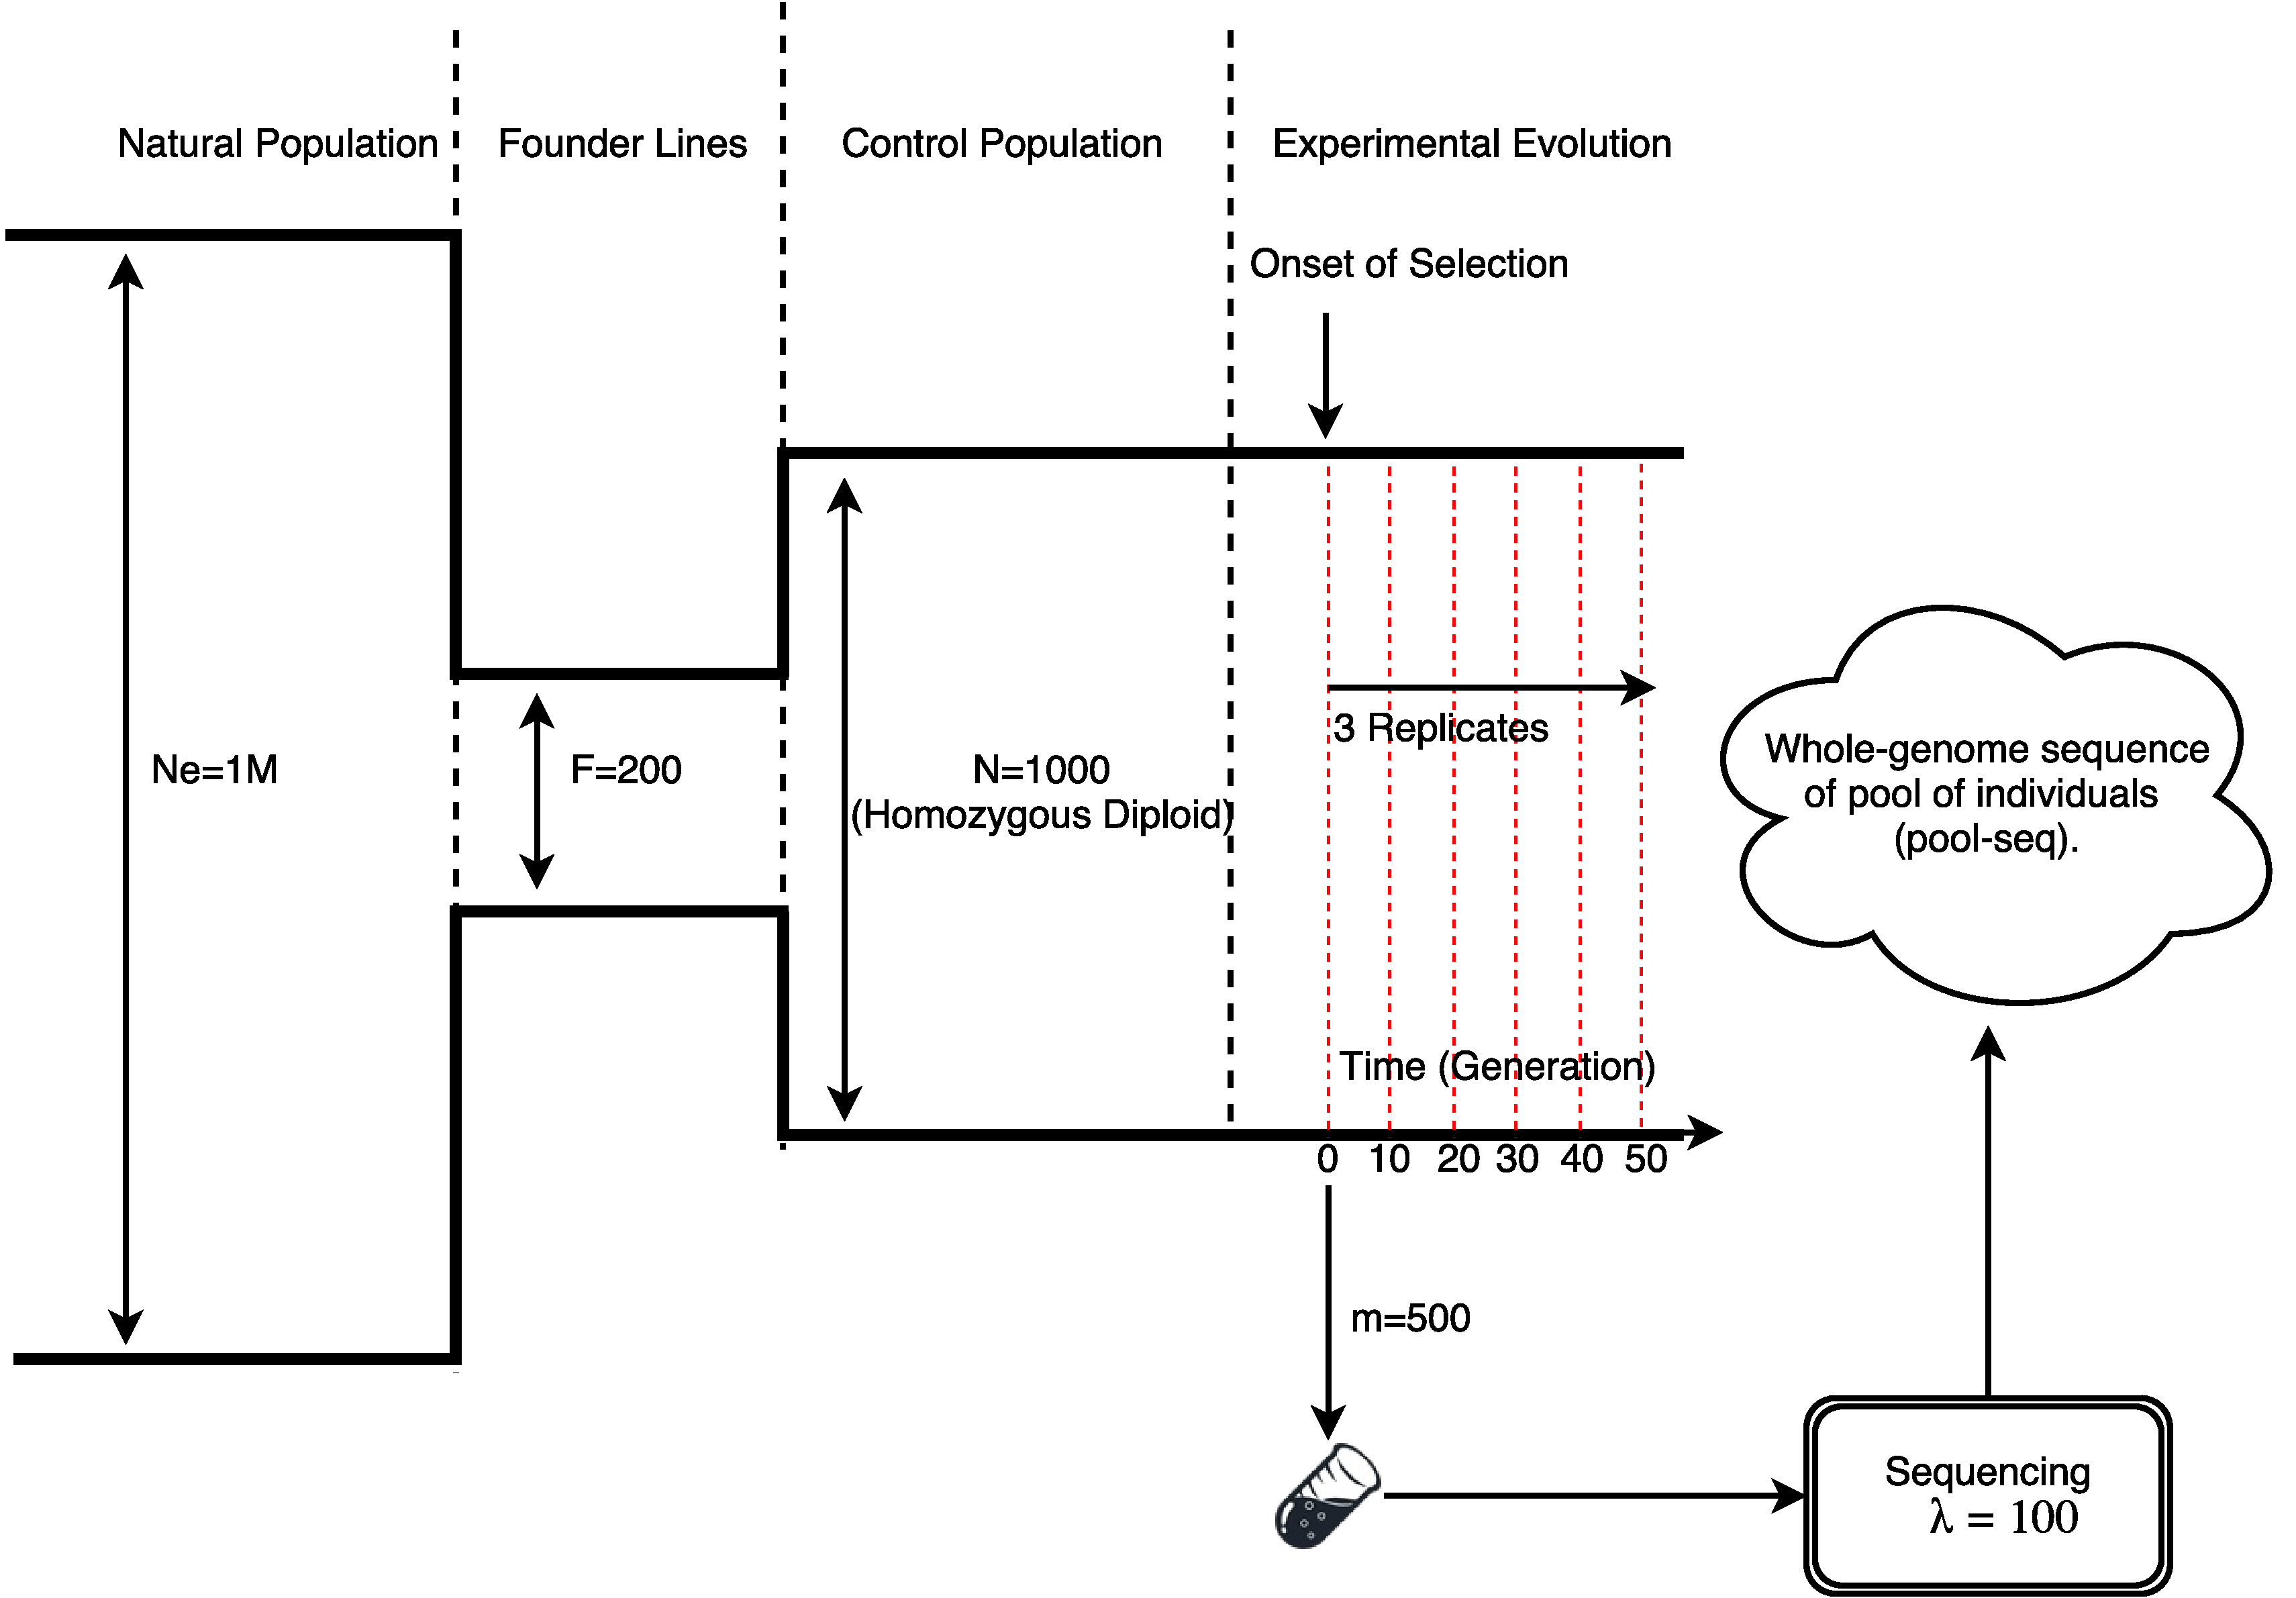
\includegraphics[trim=0.1in 0 .08in 0.02in , 
	clip,width=\textwidth]{figures/ExperimentalEvolution.pdf}
	\caption{ {\bf Two different settings for collecting genomic time series 
	data.}
Tow different setting in which dynamic data is collected is depicted with 
typical parameters of Drosophila Melanogaster. In both settings 6 samples 
(vertical red dashed lines) are taken every 10 generation.
When sampling from naturally evolving populations (A), the onset of selection 
is unknown, population size is larger. For (controlled) experimental evolution, 
first founder lines are sampled from natural population to create a homogenous 
population. Multiple replicates of the curated population is evolved and 
sampled thought time.
 } 
	\label{fig:ee}
\end{figure}


\begin{figure}[H]
	\centering
	\includegraphics[width=\textwidth]{figures/{markovDists}.pdf}
              \caption{{\bf Comparison of empirical distributions of
                  allele frequencies (green) versus predictions from
                  Brownian Motion (red), and Markov
                  Chain (blue).} Panels A-F: Experiments were conducted
                under neutral evolution with different starting
                frequencies $\nu_0\in\{0.005,0.1\}$ and sampling times
                $\tau \in \{1,10,100\}$ generations. The empirical
                distribution was computed by sampling 143,900 sites
                with $\nu_0=0.005$ and 47,500 with variants
                $\nu_0=0.1$.  computed from neutrally evolving
                simulations is depicted in green lines. Panels G,H,I:
                Comparisons of Empirical and Markov chain based
                predicted allele frequency value distributions under a
                selection regime with $s=0.1$. Initial frequency was
                chosen as $\nu_0=0.005$ and sampling performed after
                $t=\{1,10,100\}$ generations.}
	\label{fig:markov}
\end{figure}

\begin{figure}[H]
	\centering
	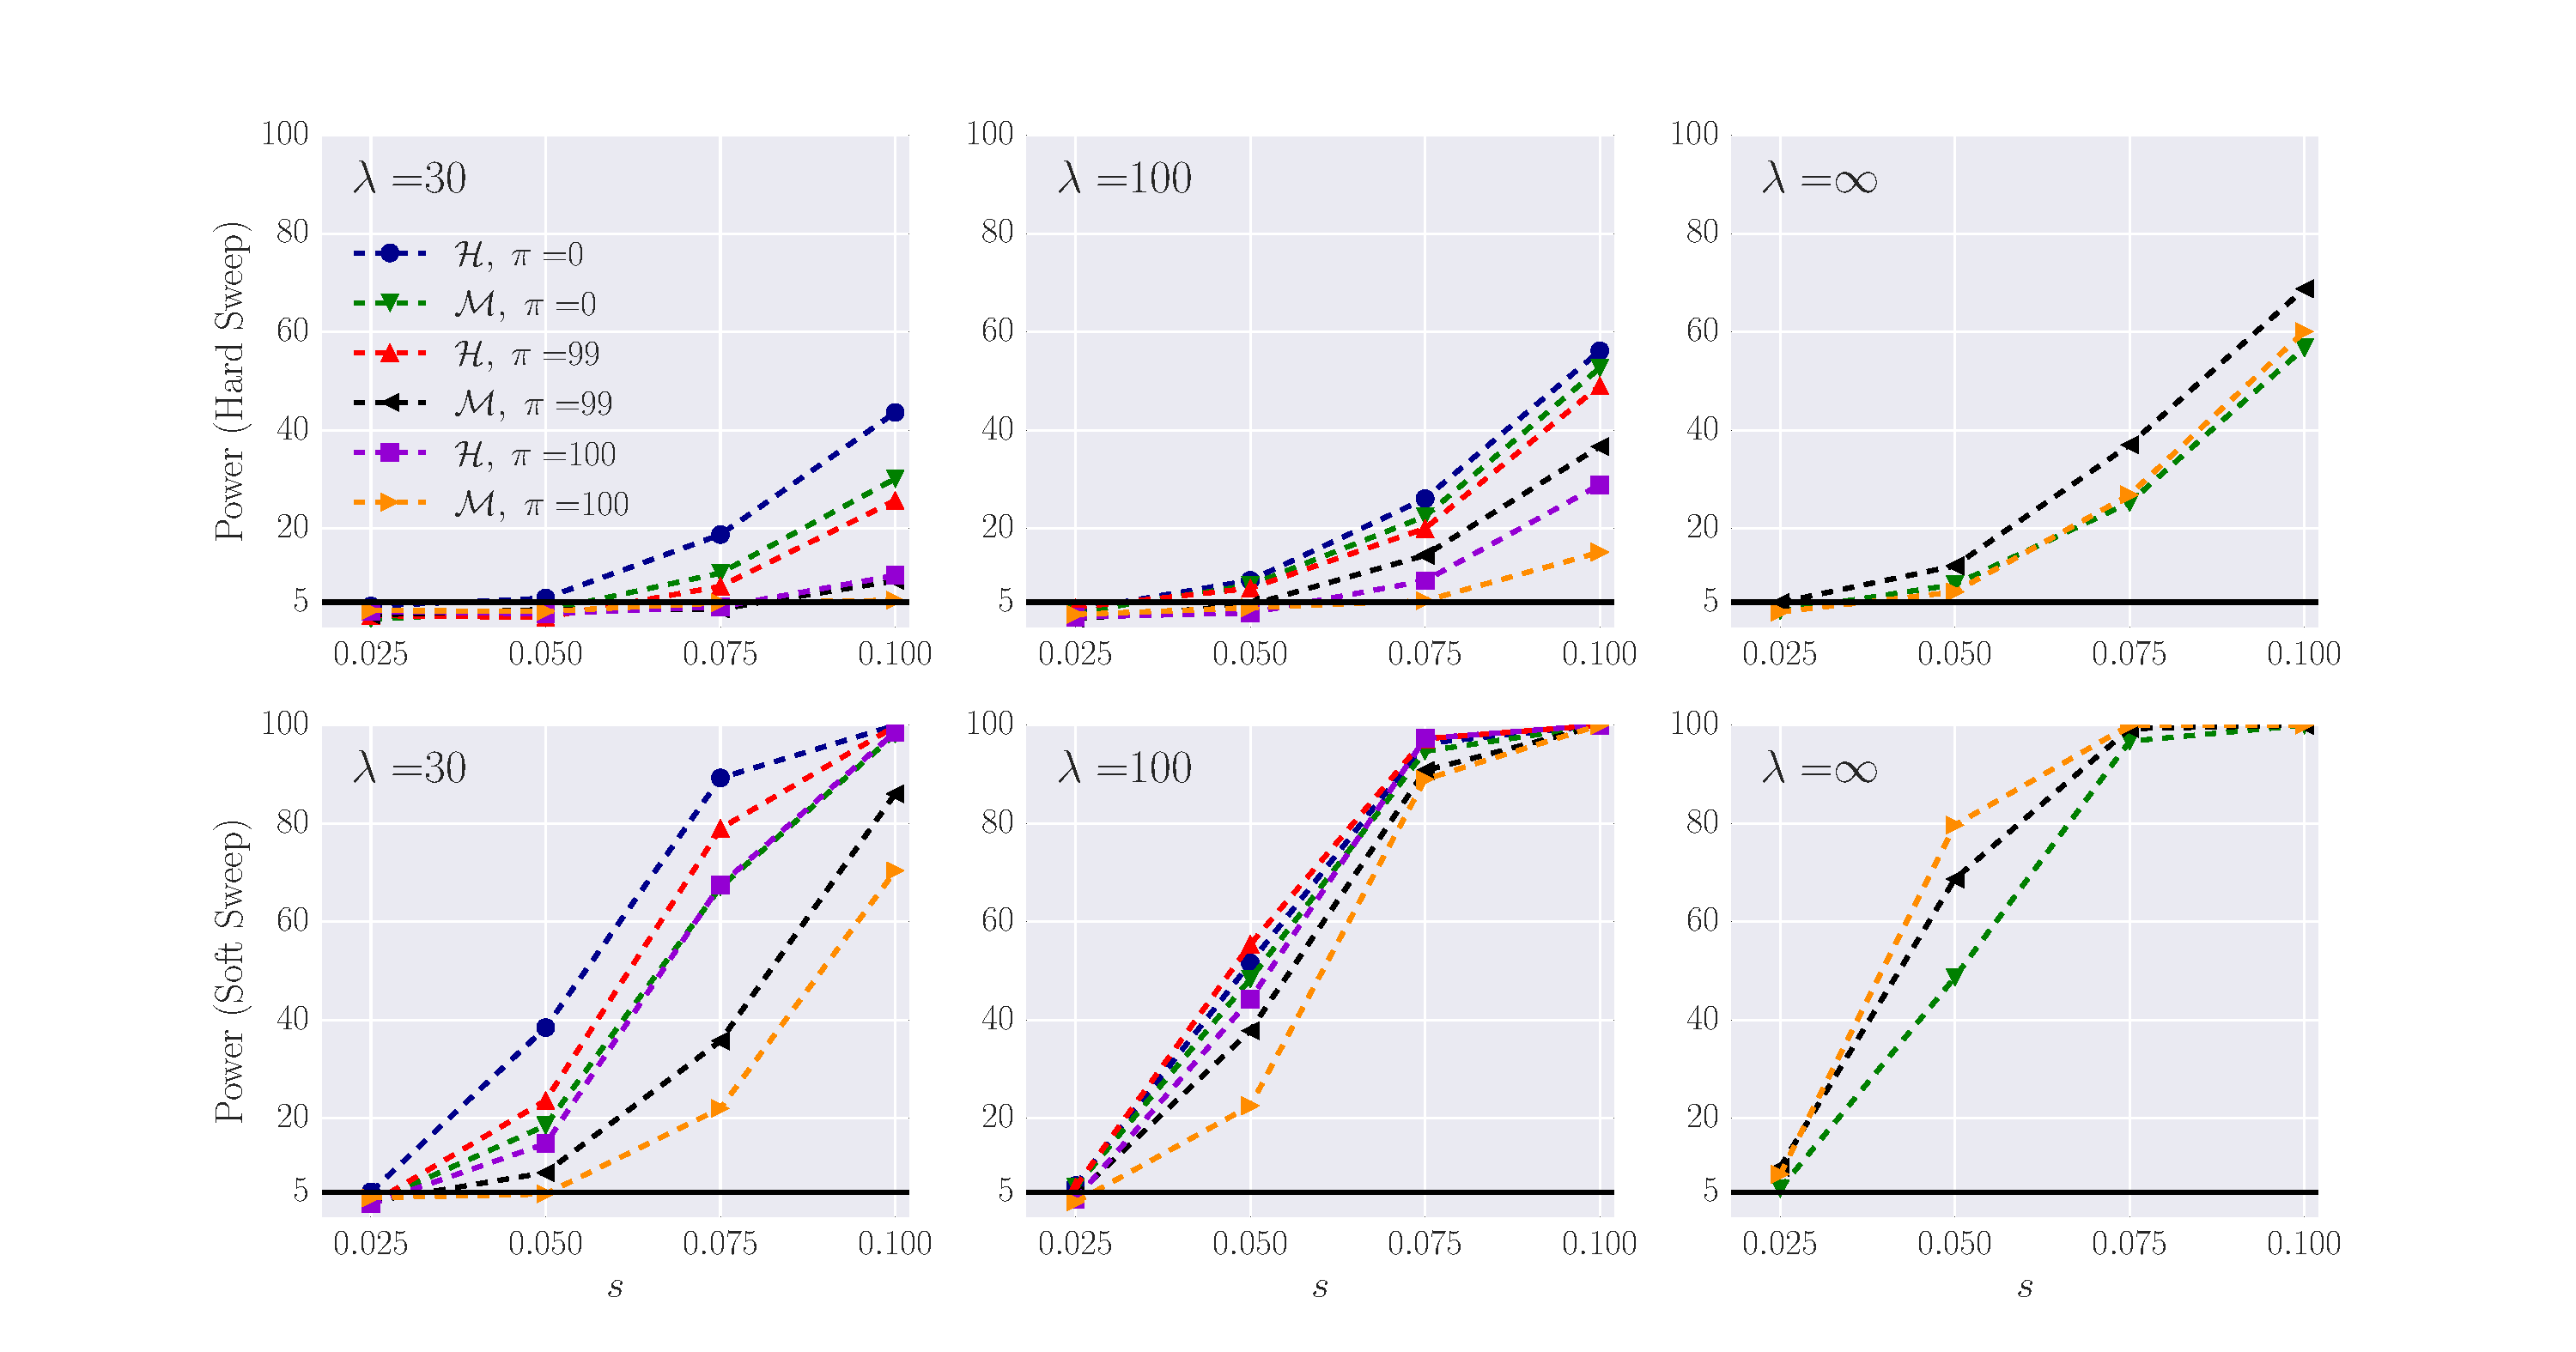
\includegraphics[width=\textwidth]{figures/powerCLR.pdf}
	\caption{{\bf Detection power for Markov chain and HMM with
            different composite statistics.}  Detection power for
          Markov chain ($\Mc$) and HMM ($\Hc$) under hard sweep (top)
          and soft sweep (bottom), for different coverage $\lambda$
          and selection strength $s$.  Each point represent power,
          scaled area under ROC curve when FPR $\le$0.05, of 1000
          simulations of 50Kbp regions with default parameter setting.
        } \label{fig:powerCLR}
\end{figure}

\begin{figure}[H]
	\centering
	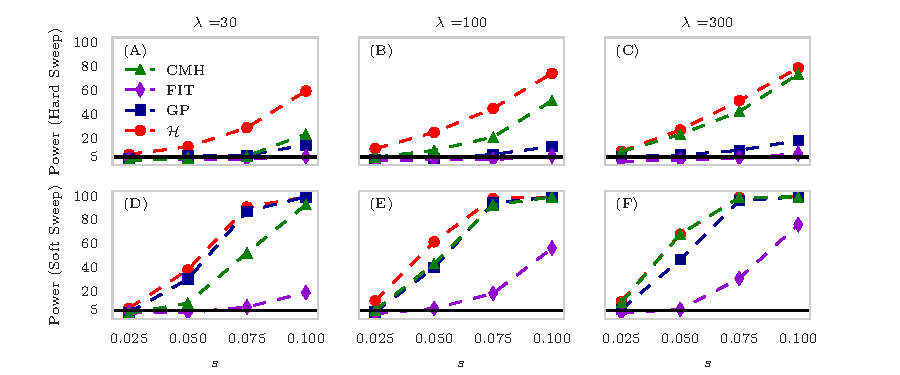
\includegraphics[width=\textwidth]{figures/power.pdf}
	\caption{ {\bf Power calculations for detection of selection.}
          Detection power for \comale ($\Hc$), Frequency Increment
          Test (FIT), Gaussian Process under hard sweep (top) and soft
          sweep (bottom), for different coverage $\lambda$ and
          selection strength $s$.  Each point represent power, scaled
          area under ROC curve when FPR$\le$0.05, of 1000
          simulations.} \label{fig:power}
\end{figure}

\clearpage
\newpage
\begin{figure}[H]
	\centering
	\includegraphics[width=0.75\textwidth]{figures/{runTime.pdf}}
	\caption{{\bf Running time}. Box plot of running times
        (cpu-secs.) of \comale, HMM, GP with single, 3, 5, 7, and 10
        loci over 1000 simulations conducted on a workstation with
        4th Generation Intel Core i7 processor. The average running time 
        for each method
        is shown on the x-axis.}
	\label{fig:runTime}
\end{figure}
\clearpage
\newpage

\begin{figure}[H]
	\centering
	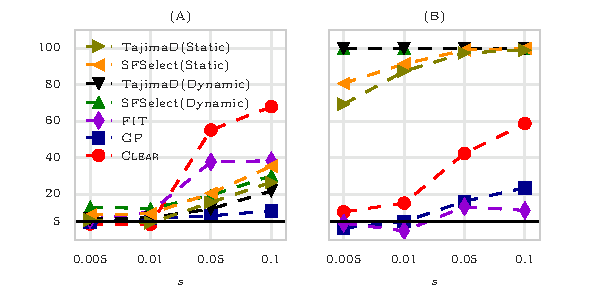
\includegraphics[width=0.7\textwidth]{figures/naturalee.pdf}
	\caption{{\bf power of SFS based statistics.} Power, area under ROC curve 
	when FPR$\le$0.05, for detecting
          selection in a 50Kbp region for Frequency Increment Test
          (FIT), Gaussian Process (GP), \comale\ ($\Hc$) on 200 simulations 
          hard-sweep
          natural experimental evolution with $N_e=10^4$ and depth 
          $\lambda=\infty$, for each of
          selection strength $s$. 
          In this experiment start of sampling
          is random, then 5 samples are taken every 10
          generations. (a) Start of sampling is chosen randomly
          throughout the sweep $\tau_1 \sim
          U\left[1,t_{\nu=1}(s,N_e)\right]$ (left) and chosen in the
          finale of the sweep $\tau_1 \sim
          U\left[t_{\nu=0.9}(s,N_e),t_{\nu=1}(s,N_e)\right]$ (right),
          where $t_{\nu=x}(s,N_e)$ to be understood as the number of
          expected generations required to reach carrier frequency $x$
          in a hard sweep and $U[a,b]$ is discrete uniform
          distribution.} \label{fig:powerSFS}
\end{figure}

\clearpage
\newpage
\begin{figure}[H]
	\centering
	\includegraphics[trim=.2in 0 .2in 0, 
	clip,width=\textwidth]{figures/{rank100.0}.pdf}
	\caption{Cumulative Distribution  Function (CDF) of the distribution of the rank of the adaptive allele in 500 simulations for Markov Chain ($\Mc$), Gaussian Process (GP) and Frequency Increment Test (FIT), for different values of selection strength $s$ and initial carrier frequency. Area Under Curve (AUC) is computed as a quantitative measure ranking performance of methods for each configuration.}
	\label{fig:rank}
\end{figure}

\clearpage
\newpage
\begin{figure}[H]
	\centering
(A)	\\ \includegraphics[width=0.7\textwidth]{figures/{bias.30}.pdf} \\
(B)\\	\includegraphics[width=0.7\textwidth]{figures/{bias.100}.pdf}\\
(C)\\	\includegraphics[width=0.7\textwidth]{figures/{bias.inf}.pdf}
	\caption{Distribution of bias ($s-\hat{s}$) over 500 simulations for each 
	value of strength of selection $s$ and starting carrier frequency $\nu_0$. 
	Results for when coverage $\lambda=30,100,\infty$ is shown in panels (A), 
	(B), (C), respectively.} 
	\label{fig:bias}
\end{figure}

\clearpage
\newpage
\begin{figure}[H]
	\centering
	\includegraphics[width=\textwidth]{figures/{manhattan.min500snp}.pdf}
	\caption{Manhattan plot of the composite $\Hc$ statistic (top)
          and the number of SNPs (bottom) in 50Kbp sliding window with
          steps of 10Kbp, excluding windows with less that 500
          SNPs. Regions in which their $\Hc$ statistic falls in top
          one percentile distribution is denoted with red
          color. Pearson correlation between the number of SNPs and $\Hc$ of 
          all windows
          is -0.09 and for the candidate regions is -0.08.  This
          indicates the spurious effect of windows with low diversity
          is removed from out study (potentially at cost of some false
          negatives). See Fig.~\ref{fig:manhattan}.}
	\label{fig:manhattancutoffed}
\end{figure}

\clearpage
\newpage

\section*{Tables}
\begin{table}[H]
	\begin{tabular}{c}
		\centering \begin{tabular}{c|c|p{3in}|c|c|c}
Rank	&GO ID	&GO Term	&-log($p$-value)	&Hits	&Num of Genes\\\hline
1	&GO:0004046	&aminoacylase activity	&9.7	&5	&7\\
2	&GO:0006520	&cellular amino acid metabolic process	&6.4	&5	&18\\
3	&GO:0015101	&organic cation transmembrane transporter activity	&6.4	&3	&5\\
4	&GO:0007501	&mesodermal cell fate specification	&6.2	&4	&11\\
5	&GO:0004601	&peroxidase activity	&5.1	&4	&17\\
6	&GO:0006979	&response to oxidative stress	&5.0	&8	&79\\
7	&GO:0007483	&genital disc morphogenesis	&4.7	&2	&4\\
8	&GO:0045664	&regulation of neuron differentiation	&4.7	&2	&4\\
9	&GO:0045787	&positive regulation of cell cycle	&4.3	&2	&5\\
10	&GO:0008074	&guanylate cyclase complex, soluble	&4.3	&2	&5\\
11	&GO:0009312	&oligosaccharide biosynthetic process	&4.2	&3	&13\\
12	&GO:0004653	&polypeptide N-acetylgalactosaminyltransferase activity	&4.1	&3	&14\\
13	&GO:0070864	&sperm individualization complex	&4.0	&2	&6\\
14	&GO:0008324	&cation transmembrane transporter activity	&4.0	&2	&6\\
15	&GO:0008599	&protein phosphatase type 1 regulator activity	&4.0	&2	&6\\
16	&GO:0008378	&galactosyltransferase activity	&3.8	&2	&7\\
17	&GO:0007492	&endoderm development	&3.8	&2	&7\\
18	&GO:0000302	&response to reactive oxygen species	&3.8	&2	&7\\
19	&GO:0040014	&regulation of multicellular organism growth	&3.6	&3	&18\\
20	&GO:0016485	&protein processing	&3.5	&3	&19\\
21	&GO:0006030	&chitin metabolic process	&3.5	&7	&99\\
22	&GO:0020037	&heme binding	&3.4	&8	&127\\
23	&GO:0005815	&microtubule organizing center	&3.4	&2	&9\\
24	&GO:0042659	&regulation of cell fate specification	&3.4	&2	&9\\
25	&GO:0007415	&defasciculation of motor neuron axon	&3.4	&2	&9\\
26	&GO:0045297	&post-mating behavior	&3.2	&2	&10\\
27	&GO:0010212	&response to ionizing radiation	&3.2	&2	&10\\
28	&GO:0007519	&skeletal muscle tissue development	&3.2	&2	&10\\
29	&GO:0051865	&protein autoubiquitination	&3.2	&2	&10\\
30	&GO:0006182	&cGMP biosynthetic process	&3.2	&2	&10\\
31	&GO:2000134	&negative regulation of G1/S transition of mitotic cell cycle	&3.1	&2	&11\\
32	&GO:0044212	&transcription regulatory region DNA binding	&3.1	&2	&11\\
33	&GO:0040015	&negative regulation of multicellular organism growth	&3.1	&2	&11\\
34	&GO:0036011	&imaginal disc-derived leg segmentation	&3.1	&2	&11\\
35	&GO:0008061	&chitin binding	&3.1	&7	&113\\
36	&GO:0004702	&receptor signaling protein serine/threonine kinase activity	&3.0	&3	&26\\
\end{tabular}

	\end{tabular}
	\caption{Gene set enrichment of 243 genes within 25 intervals under 
          selection using Fisher exact test.}\label{tab:Fisher}
\end{table}
\clearpage
\newpage


%\section*{References}
\bibliographystyle{plain}
%bibliographystyle{Vanc5ouver}
\bibliography{library}

%%%%%%%%%%%%%%%%%%%%%%%%%%%%%%%%%%%%%%%%%%%%%
%%%%%%%%%%%%%%%%%%% Supplemental Material%%%%
%%%%%%%%%%%%%%%%%%%%%%%%%%%%%%%%%%%%%%%%%%%%%
\clearpage
%\newpage
%\setcounter{page}{1}
\setcounter{figure}{0}
\setcounter{table}{0}
\setcounter{equation}{0}
\renewcommand{\thefigure}{S\arabic{figure}}
\renewcommand{\thetable}{S\arabic{table}}
\renewcommand{\theequation}{S\arabic{equation}}

%\section*{Main text figure captions}
%\section*{Supporting information captions}
\section{Appendix}
\subsection{Approximate logistic for allele frequency} \label{app:af}
In this part we show that the dynamic of the beneficial allele can be modeled 
via a logistic function, when directional selection is the case ($h=0.5$). By 
taking derivative of Eq.~\ref{eq:transition} we have
\beq
\frac{\bfd \nu_t}{\bfd t} = \frac{s\nu_t(1-\nu_t)}{2+2s\nu_t}
\eeq
which is a differential equation that is difficult to solve. However if take 
the approximation $2+2s\nu_t \approx 2$, it becomes an 
ordinary differential equation that can be readily solved
\begin{equation}
\nu_t =\frac{1}{1+\frac{1-\nu_0}{\nu_0}e^{-st/2}} = \sigma(st/2+\eta(\nu_0)) 
\label{eq:inf-pop}
\end{equation}
where $\sigma(.)$ is the logistic function and $\eta(.)$ is logit function 
(inverse of the logistic function). 

\subsection{Dynamic of Tajima's D}\label{app:td}
In this part we derive dynamic of Tajima's $D$ statistic in \emph{hard sweep} 
as function of its 
value at the onset of selection, $D_0$, selection strength and the frequency of 
the beneficial allele at the onset of selection.
Let $D_0, \Pi_0, W_0$, be Tajima's D, Tajima's estimate of  $\theta$, and 
Watterson's estimate of $\theta$ at time zero and $D_0=\Pi_0 - W_0$.
In order to compute, $D_t=\Pi_t - W_t$ we compute $\Pi_t$ and $W_t$ separately 
as follows. Let $P$ be the $n \times n$ matrix of pairwise heterozygosity if 
individuals, 
then $\Pi=\frac{1}{n^2}\sum P_{ij}$. So, if the population consist of $\nu n$ 
identical carrier haplotype (due to lack of recombination), their pairwise 
hamming distance is zero and should be subtracted from the total $\Pi_t$:
\beq
\Pi_t&= (1-\nu_t^2)\Pi_0 \label{eq:tdt0}
\eeq

To compute $W_t$, first remember that $W_t= \frac{m_t}{S_n}$ where $m_t$ is the 
number of segregating sites at time $t$ and $S_n= \sum_i^n 1/i \approx 
\log(n)$. Also we have
\beq
\frac{W_t}{W_0}&=\frac{\frac{m_t}{S}}{\frac{m_0}{S}} \ \ \Rightarrow 
W_t=\frac{m_t}{m_0}W0 \label{eq:tdt1}
\eeq
Because of hard sweep and lack of recombination assumption, the population 
at time $t$ consist of $(1-\nu_t)n$ non-carrier haplotypes and $\nu_tn$ 
identical carrier haplotypes. Since the identical carrier haplotypes does not 
contribute to the $m_t$ more than any single of them, here the number of 
segregating sites is 
equal to the sample of $(1-\nu_t)n+1$ individuals from a naturally evolving 
population.  
\AI{Reading it again, I just realized that this assumption is not entirely true.
	The noncarier haplotypes does not under go neutral evolution. They are 
	under (soft sweep) negative selection. So $m_t$ is not right.
	}
Therefore, we have
\beq
\frac{m_t}{m_0}&=\frac{\log\left((1-\nu_t)n +1 \right)\theta}{\log(n)\theta} 
\approx  
\frac{\log\left((1-\nu_t)n\right)}{\log(n)} = \frac{\log(1-\nu_t)+\log(n)}{\log(n)} = 
1+ \frac{ \log(1-\nu_t)}{\log(n)}. \label{eq:tdt2}
\eeq
Finally, by putting Eqs.~\ref{eq:tdt0},~\ref{eq:tdt1},~\ref{eq:tdt2} together, we 
can explicitly write the dynmics of $D$ statistic as
\beq
D_t&= (1-\nu_t^2)\Pi_0 - (1+ \frac{ \log(1-\nu_t)}{\log(n)} ) W_0 \\&= 
D_0-\log(1-\nu_t) \frac{W_0}{\log(n)} -\nu_t^2 \Pi_0\\
&\approx D_0-\log(1-\sigma(st/2+\eta(\nu_0))) \frac{W_0}{\log(n)} 
-\sigma(st/2+\eta(\nu_0))^2
\Pi_0.
\eeq
where $\sigma$ and $\eta$ are logistic and logit functions.


\subsection{Dynamics of Fay and Wu's H}\label{app:h}
%\bl
In any finite population size of $n$ with $m$ segregating sites, 
allele frequencies take 
discrete values, i.e.,  $x_j \in 
\{\frac{1}{n},\frac{2}{n},\ldots,\frac{n-1}{n}\}, \ \forall j \in{1,\cdot,m}$ 
and we can write
\beq
\|\bfx\|^2= \sum_{j=1}^{m} x_j^2 = 
\sum_{i=1}^{n-1}\left(\frac{i}{n}\right)^2\xi_i= 
\frac{ (n-1)}{2n}H 
\eeq
where $\xi_i$ is the number of sites with frequency $i/n$ and $H$ is the 
Fay \& Wu's estimate of $\theta$ and $\bfx \in (0,1)^m$ is the vector of allele 
frequency of a region with $m$ segregating sites.
%\el

Recently, Ronen \emph{et al.}~\cite{ronen2015predicting} devised the $1\dHAF$ 
statistic for identifying selection on static data, which has the expected 
value related to the $\|\bfx\|^2$:
\begin{equation} 
\Ebb[1\dHAF(t)]= n\| \bfx_t\|^2\approx ng(\nu_t)
\end{equation} 
where
\beq
g(\nu_t)= \theta \nu_t \left(\frac{\nu_t+1}{2} - \frac{1}{(1-\nu_t)n+1}\right) +
\theta (1-\nu_t)\left(\frac{n+1}{2n}-\frac{1}{(1-\nu_t)n+1}\right)
\label{eq:hafscorepooled}
\eeq
where easily follows that
\beq
\theta_H(t)=\frac{n-1}{2} g(\nu_t)
\eeq
\subsection{Greedy computation of time-series SFS-based  
statistics}\label{app:agg}
As discussed in Section~\ref{sec:extending-sfs}, modeling dynamic of Tajima's 
$D$ (and Fay\&Wu's $H$) requires knowledge of initial carrier frequency $\nu_0$ 
and the value of $D$ (and $H$) statistic at the onset of selection, which are 
often unknown.
As these statistics are monotonously decreasing (or increasing for SFSelect) 
under no demographic changes, we chose to greedily aggregate statistics 
throughout time. For example, for Tajima's $D$, we have 
\beq
\Dc = \sum_{t \in \Tc} D_t
\eeq
where the same procedure applies to Fay\&Wu's $H$ and SFSelect.


\subsection{Linkage Disequilibrium}
Nonrandom associations, Linkage Disequilibrium (LD), between 
polymorphisms are established in the 
substitution process, broken by recombination events 
and reinforced by selection. 
Although LD can not be measured in pooled sequencing data (phased 
haplotype data is required), it is still worthwhile 
to examine the behavior of LD as a result of the interaction between 
recombination and natural selection. In this part we theoretically overview 
expected LD in short EEs.

Let $\rho_0$ be the LD at time zero between the beneficial allele and a 
segregating site $l$ base-pairs away, then under natural selection we have
\beq
\rho_t= \alpha_t\beta_t \rho_0=e^{-rtl} \left(\frac{H_t}{H_0}\right)  
\rho_0\label{eq:ldt}
\eeq
where $H_t=2\nu_t(1-\nu_t)$ is the heterozygousity at the selected site, $r$ is 
the recombination rate/bp/gen. The 
\emph{decay factor}, $\alpha_t=e^{-rtl}$,
and \emph{growth factor}, $\beta_t$ (see Eq. 30-31 in 
\cite{Stephan2006The}), are result of recombination and 
selection, respectively. Fig.~\ref{fig:ld3d} presents the expected theoretical 
value of LD when $\rho_0=0.5$ between beneficial allele (site at position 500K) 
and the rest of 
genome, and $\nu_0=0.1$. For neutral evolution (top), LD decays exponentially 
through space and time, while in natural selection (bottom), LD increases and 
then decreases. Interestingly, LD increases to its maximum value, 1, for the 
nearby region (the plateau in the Fig.~\ref{fig:ld3d} bottom) of the beneficial 
allele.

In principle, LD increases after the onset of selection, until $\log(\alpha_t) 
+\log(\beta_t) 
>0$, see Eq.~\ref{eq:ldt}. 
Specifically, log of decay term is linear and, using 
Eq.~\ref{eq:inf-pop}, we write growth 
factor in term of initial frequency $\nu_0$ and selection strength $s$. 
Fig.~\ref{fig:ldf} depicts interaction of decay and growth factors for weak and 
strong selection and soft and hard sweeps. In all the case, LD of the 
beneficial allele with a segregating site 50Kbp away, increases in the first 50 
generations, which give rise to increasing number of \emph{hitchhikers}. 

Increase of LD in a large (100Kbp) region is particularly advantageous to the 
task of identifying the region under selection, if the composite statistics is 
used. As a result, $\Hc$ statistic outperforms existing (single-loci) tools in 
identifying selection. In contrast, augmentation of LD, increases the 
number 
of candidates for 
the beneficial allele, which makes is difficult to localize the beneficial 
allele.

\newpage
\section{Supplemental Figs. and Tables}
\begin{figure}[H]
	\centering
	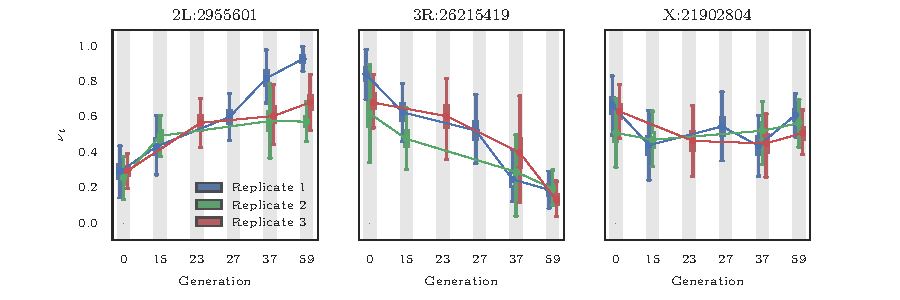
\includegraphics[width=\textwidth]{figures/trajectoryReal.pdf}
	\caption{{\bf Dynamic pool-sequenced data trajectory.} Trajectory of three 
	different variants which evidently raise in frequency. Note that for read 
	count data allele frequency is hidden. Here we draw the posterior  
	distribution of the allele frequency at each time point using box plot. The 
	median of each distribution is denoted by dots and the variance of each box 
	is inversely related to the depth of the measurement.
	sites.} 
	\label{fig:trajectoryReal}
\end{figure}

\begin{figure}[H]
	\centering
	\includegraphics[trim=.0in 0 .0in 0, 
	clip,width=0.5\textwidth]{figures/{statePosterior}.pdf}
	\caption{{\bf Posterior distribution of allele frequency.} Distribution of 
	allele hidden frequency for 
		different values of depth $d=\{5,50,500\}$. In all the cases, the 
		number of 
		read counts for the derived allele is one-fifth of total depth. Dealing 
		with dynamic data (and possibly multi-replicate), each site has 
		multiple 
		measurements, that can have different depth, i.e. uncertainty.} 
	\label{fig:stateConditional}
\end{figure}
\begin{figure}[H]
	\centering
	\begin{tabular}{c}
		\includegraphics[trim=.2in 0 .0in 0, 
		clip,width=\textwidth]{figures/{depthHetero}.pdf}
	\end{tabular}
	\caption{{\bf Heterogeneous depth throughout time series data.} Read depth 
	at 
	four different sites in real data showing that ascertainment bias is 
	different for each measurement.} 
	\label{fig:depthHetero}
\end{figure}

\begin{figure}[H]
	\centering
	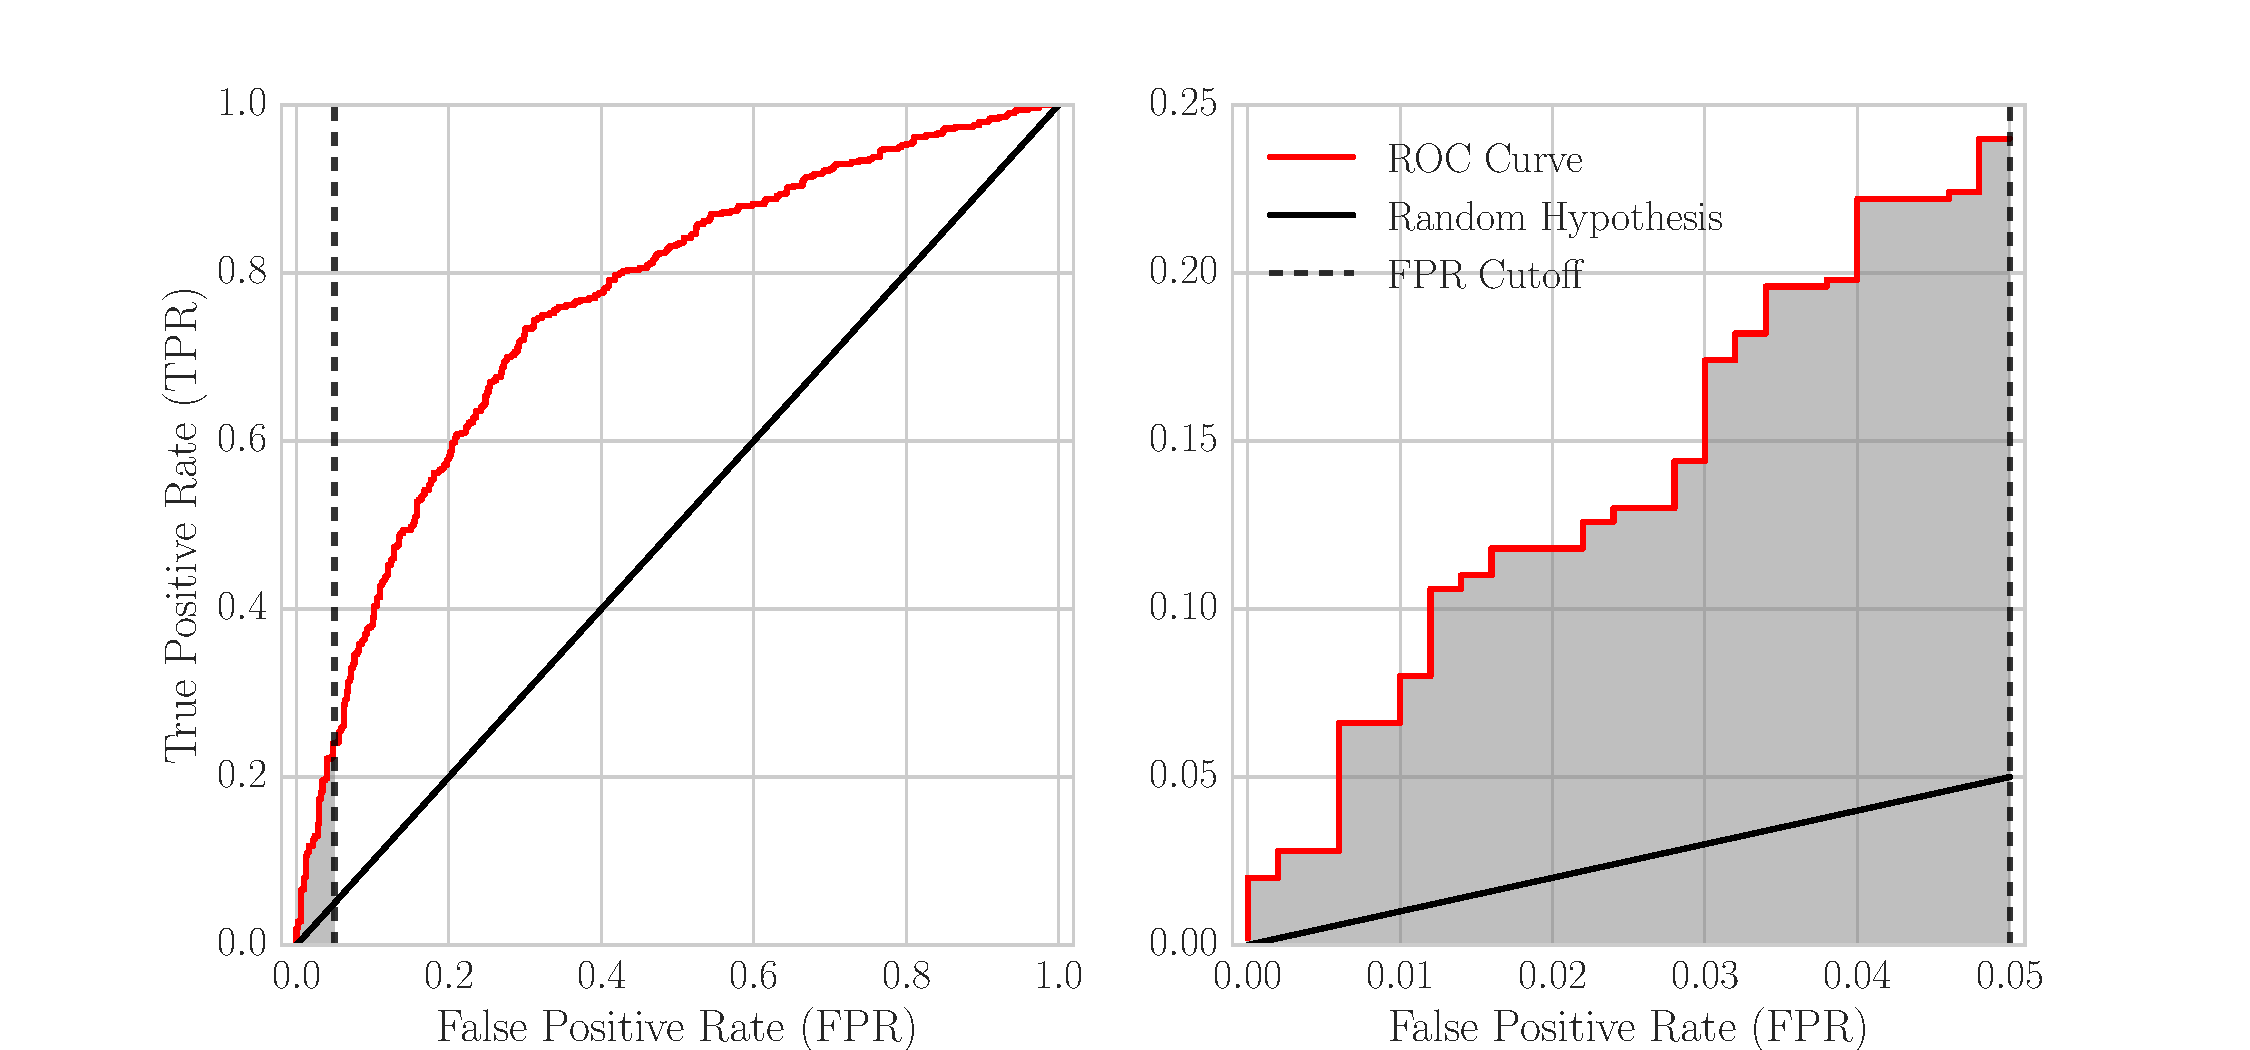
\includegraphics[trim=0.4in 0 .8in 0.02in , 
	clip,width=\textwidth]{figures/powerROC.pdf}
	\caption{{\bf Power of detecting selection.} 
		Statdard ROC curve (left) for the task of detecting selection on 1000 
		simulations (500 selection and 500 neutral). The diagonal black line 
		represents performance of a random hypothesis which achieves AUC of 
		0.5. To avoid computing AUC for the regions that FPR is high, we 
		restrict ROC curve to the regions where FPR$\le 
		0.05$ (right). In this case, we define power to be the (scaled) AUC of 
		the 
		restricted regions.} \label{fig:powerROC}
\end{figure}



\begin{figure}[H]
	\centering 
	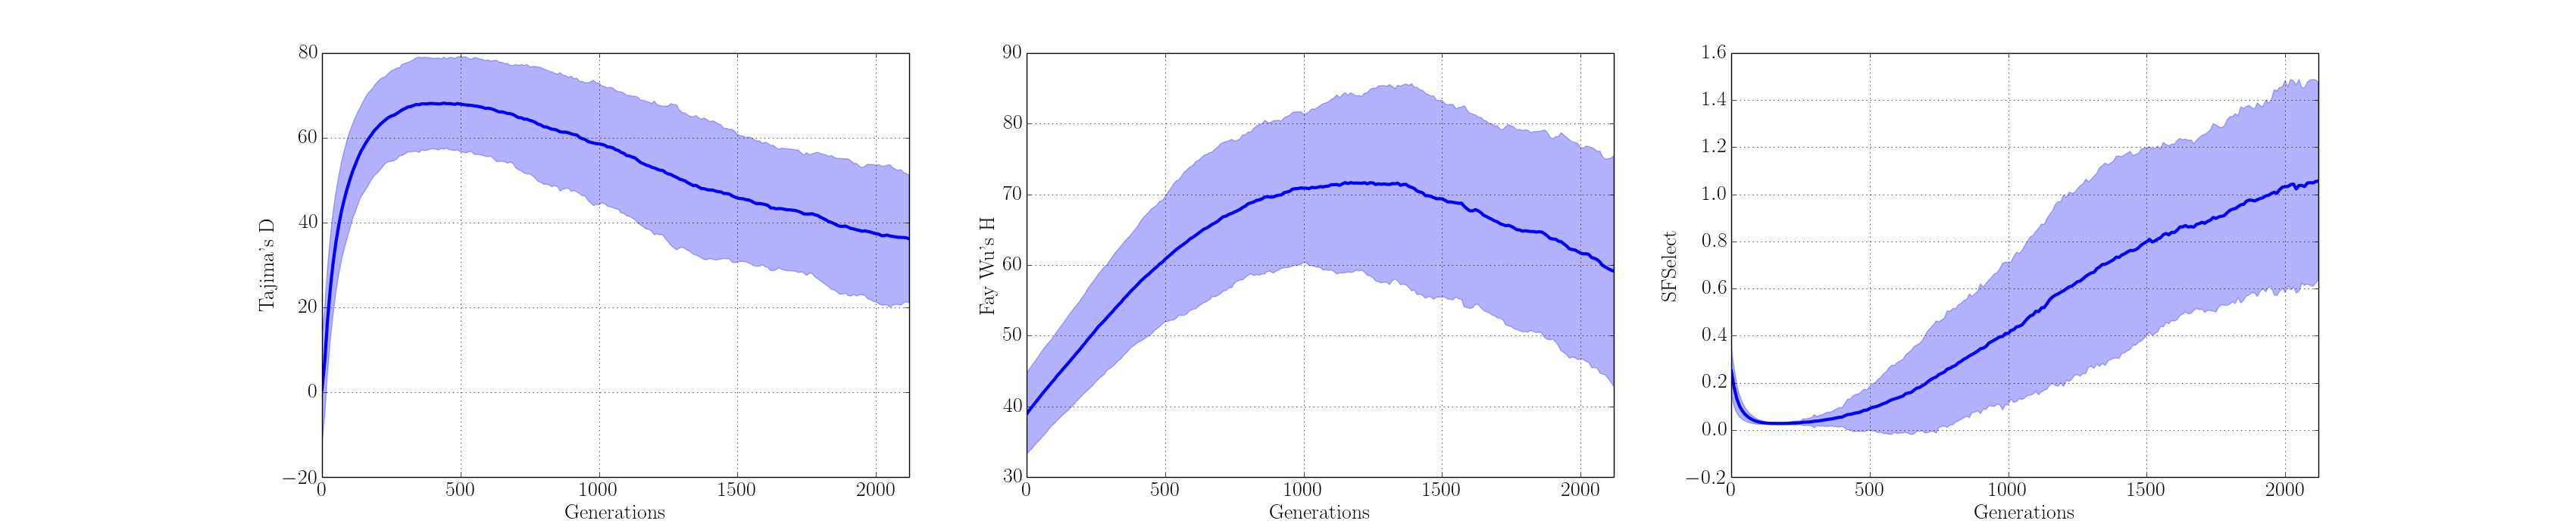
\includegraphics[trim=3.2in 0.1in 3.2in 0.2in , 
	clip,width=\textwidth]{figures/bottleneck}
	\caption{{\bf Effect of bottleneck in a typical experimental
            evolution experiment with restricted number of founder
            lines.} For the experiment, $F=200$ founders were selected
          from a larger population size ($N_e=10^{-6}$), and evolved
          under neutral scenario ($s=h=0$). The statistics for
          Tajima's D (left), Fay Wu's H (middle) and SFSelect were
          computed for 1000 neutral simulations and the mean and 95\%
          confidence interval plotted. Under neutral evolution all the 
          statistics expected to be constant throughout time and when 
          population is under selection $D$ and $H$ take negative values and 
          SFSelect take positive values. In experimental evolution, bottleneck 
          effect will suppress the signal of selection, especially in early 
          generations. }
	\label{fig:bottleneck}
\end{figure}


\begin{figure}[H]
	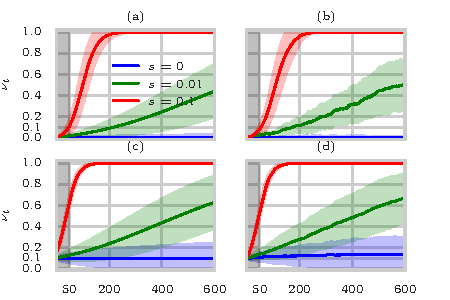
\includegraphics[trim=1in 0.1in 1in 
	0.1in,clip,width=\textwidth]{figures/AF.pdf}
	\caption{{\bf Theoretical (Markov Chain) and Empirical trajectories of 
	favored allele for hard and soft sweep scenarios}. 
		Theoretical and empirical (1000 simulations) trajectories of the 
		frequency of the favored 
		allele for experimental evolution when census (diploid) population size 
		is $1000$. In each panel $s=0$ denotes neutral (blue) evolution, 
		$s=0.01$ represents weak selection (green), and $s=0.1$ illustrates 
		strong selection, and 95\% confidence interval is shaded with the same 
		color. In all cases, A) theoretical hard sweep, B) empirical hard 
		sweep, C) theoretical soft sweep and D) empirical soft sweep the 
		theoretical model is consistent with simulations.
		Also, first 50 generation since the onset of selection, which is 
		considered to be typical sampling span for experimental evolution, is 
		shaded in gray. It is evident that sampling span is negligible to the 
		time required for fixation, even for strong selection, winch makes it 
		difficult to differentiate between neutral evolution and natural 
		selection.
}
	\label{fig:sweep}
\end{figure}

\begin{figure}[H]
	\centering
	\begin{tabular}{c}
		\includegraphics[trim=.2in 0 .0in 0, 
		clip,width=\textwidth]{figures/{depth}.pdf}
	\end{tabular}
	\caption{ {\bf Distribution of depth in the real data.}
		 Scaled PDF (A) and CDF (B) of the read depths of all ($\approx$20.1M) 
		 measurements, i.e., all replicates and time points of the all 
		 ($\approx$1.5M) variants.
		 Scaled PDF (C) and CDF (D) of the minimum depth of sites. Although 
		 most ($\approx$11.5M) of the measurements have depth of 50 or greater 
		 (dashed line in (A),(B)), only a small fraction ($\approx$10K) of 
		 variants (dashed line in (C),(D)) pass the filter of having minimum 
		 depth of 50.}  
	\label{fig:depth}
\end{figure}

\begin{figure}[H]
	\centering
	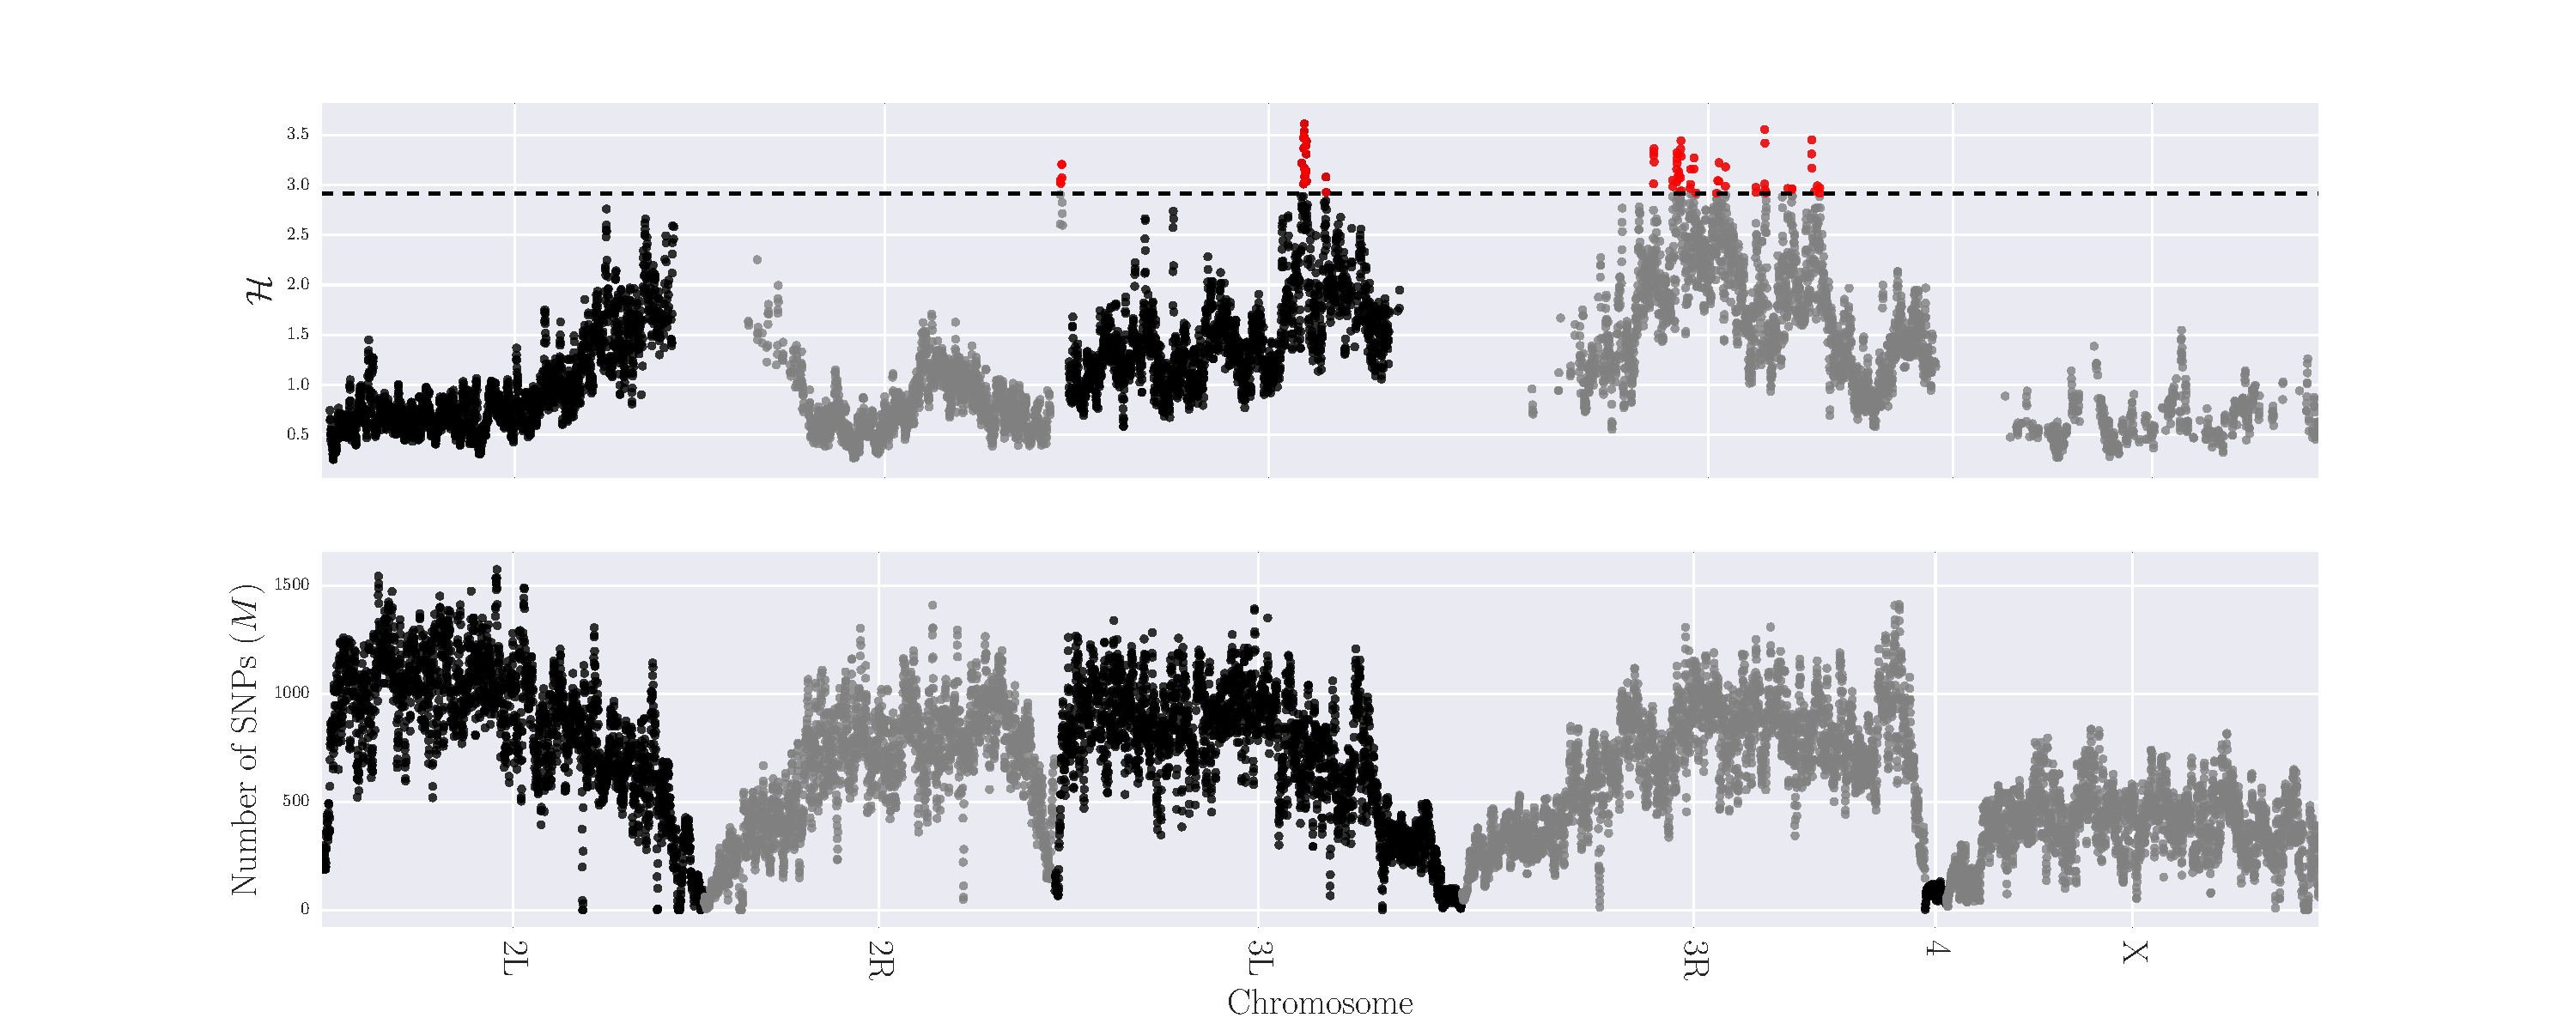
\includegraphics[width=\textwidth]{figures/manhattan.pdf}
	\caption{{\bf Manhattan plot.} Distribution of the composite $\Hc$ 
	statistic (top) 
		and the number of SNPs (bottom) for 50Kbp sliding window with steps of 
		10Kbp across genome. Regions in which their $\Hc$ statistic falls in 
		top one 
		percentile 
		distribution is denoted with red color. Pearson correlation between the 
		number of SNPs and 
		$\Hc$ of all windows is -0.03 and is -0.27 when restricting to the 
		candidate regions is -0.27. This 
		nine-fold increase in correlation implies that the $\Hc$ statistic 
		takes 
		more extreme values as the number of SNPs in the window is less than 
		expected ($\approx$1100). } 
	\label{fig:manhattan}
\end{figure}

\begin{figure}[H]
	\centering
	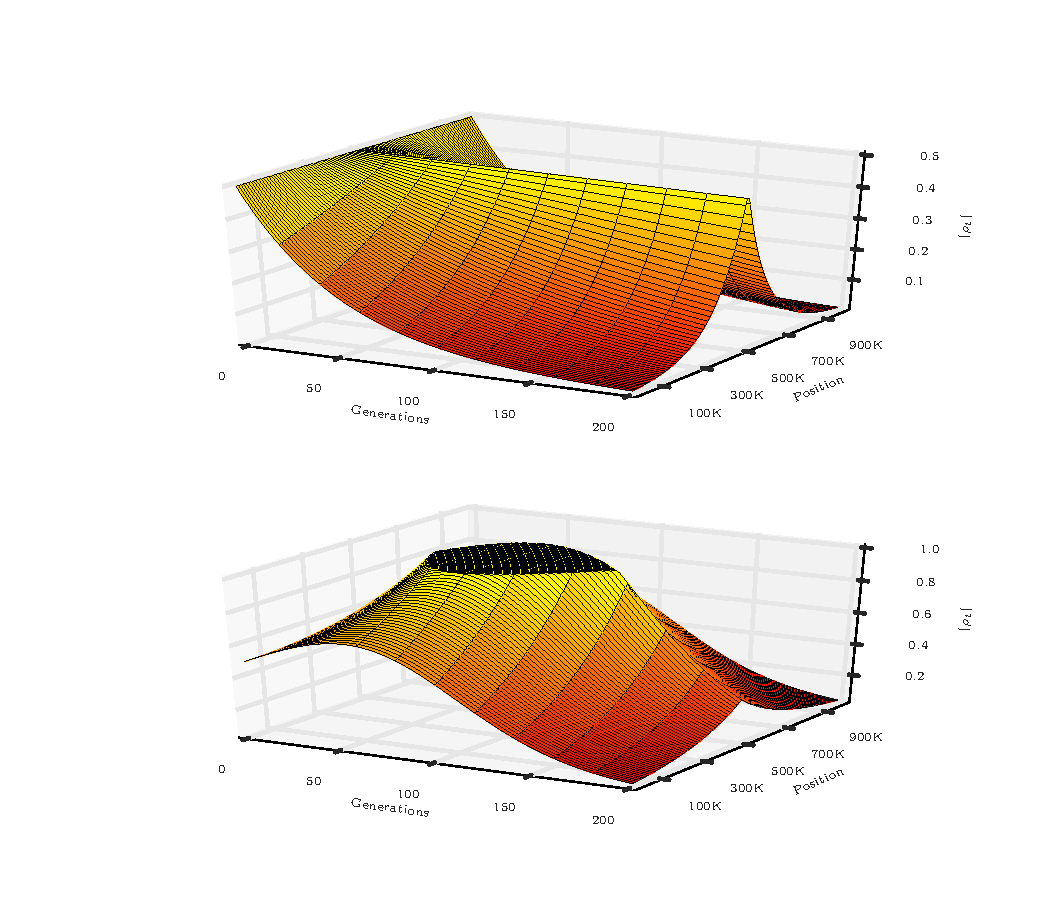
\includegraphics[width=\textwidth]{figures/LDDecay3d}
	\caption{ {Dynamic of LD.}
		Decay of LD ($|D'|$ measure) of the minimum AF site at 
		position 500K with the rest of genome in genetic drift with 
		$r=2\times10^{-8}$ (top) and hard sweep with $s=0.01$ (bottom).}	
		\label{fig:ld3d}
\end{figure}

\begin{figure}[H]
	\centering
	\begin{tabular}{l|l}
		(A)&(B)\\
		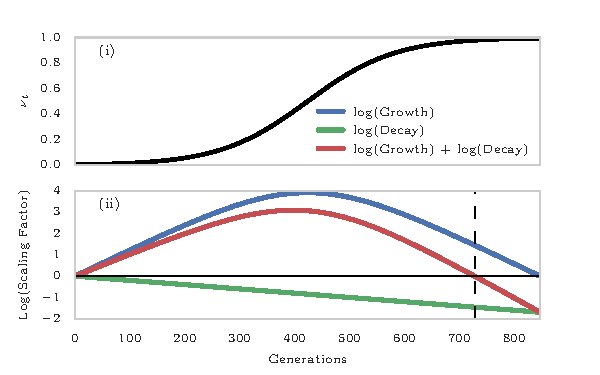
\includegraphics[width=0.5\textwidth]{figures/decayFactors0}
		&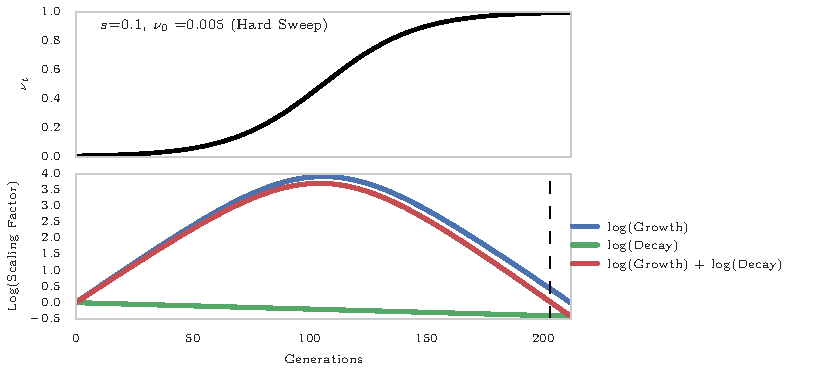
\includegraphics[width=0.5\textwidth]{figures/decayFactors1}\\
		\hline(C)&(D)\\
		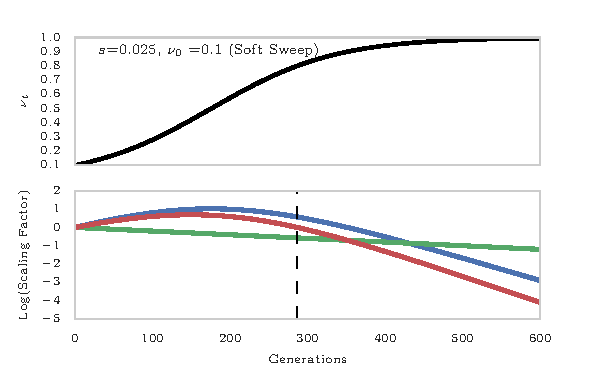
\includegraphics[width=0.5\textwidth]{figures/decayFactors2}
		&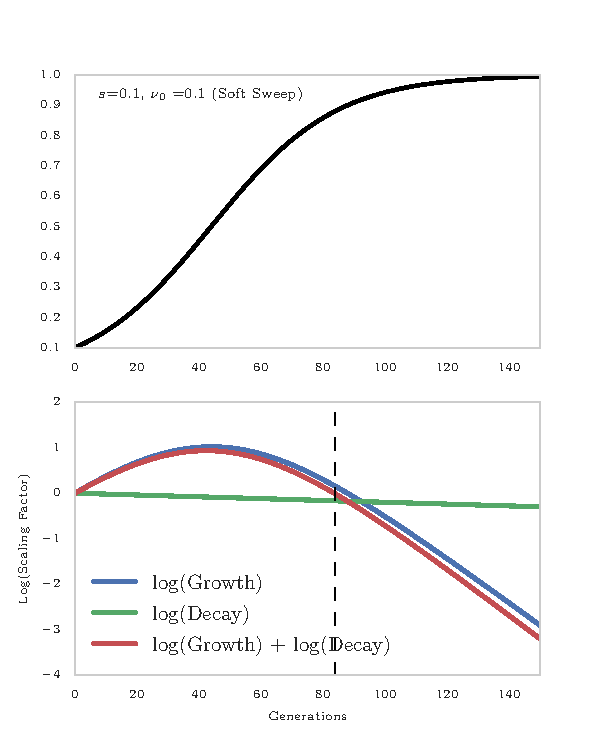
\includegraphics[width=0.5\textwidth]{figures/decayFactors3}		
	\end{tabular}
	
	\caption{{\bf Interaction between growth and decay factors of LD.}
		Expected evolution of LD under natural 
		selection for weak selection (s=$0.01$) and a distance of 100Kb between 
		sites. In this setting, after about 1000 generations LD start to decay 
		(red 
		curve).} \label{fig:ldf}
\end{figure}



\begin{figure}[H]
	\centering
	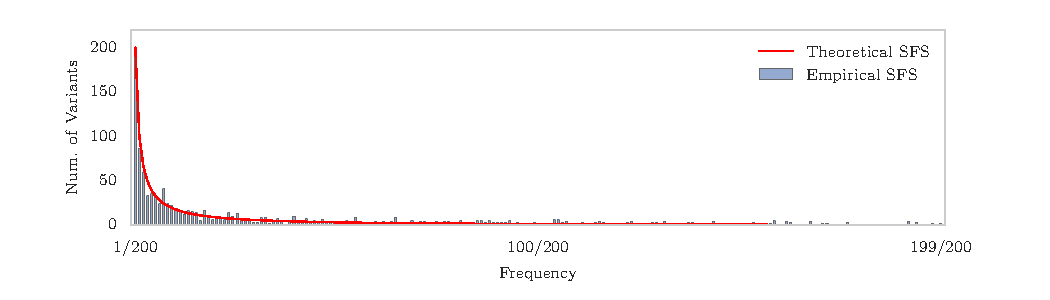
\includegraphics[trim=1in 0.1in 1in 
	0.1in,clip,width=\textwidth]{figures/sfs.pdf}
	\caption{{\bf Site Frequency Spectrum.} Theoretical and Empirical SFS for a 
	neutral population of 200 
		individuals.}	\label{fig:sfs}
\end{figure}

\begin{figure}[H]
	\centering 
	\includegraphics[width=\textwidth]{figures/{msmsts}.pdf}
	\caption{{\bf Dynamic SFS-base statistics.} Mean and 95\% CI of 100 
	simulations for neutral (blue trajectories) selection with $s=0.1$ (red 
	trajectories).}
	\label{fig:sfsts}
\end{figure}


\ignore{
\begin{figure}[H]
	\centering
	\includegraphics[trim=1.2in 0 .0in 0, 
	clip,width=\textwidth]{figures/{dominance}.png}
	\caption{Dominance for $s=0.1$.} 
	\label{fig:dominance}
\end{figure}}

\begin{table}[h]
	\centering
	\begin{tabular}{ccc}
		Hard Sweep & &Soft Sweep\\ \\  
		\centering \begin{tabular}{c|c|c}
$\lambda$	&Method	&Avg Power\\\hline
100	&$\mathcal{H}$	&30\\
$\infty$	&$\mathcal{H}$	&29\\
30	&$\mathcal{H}$	&23\\
100	&CMH	&19\\
30	&CMH	&10\\
$\infty$	&GP	&7\\
100	&GP	&7\\
30	&GP	&7\\
$\infty$	&FIT	&5\\
100	&FIT	&4\\
30	&FIT	&3\\
\end{tabular}

		&&\centering \begin{tabular}{c|c|c}
$\lambda$	&Method	&Avg Power\\\hline
100	&$\mathcal{H}$	&64\\
$\infty$	&$\mathcal{H}$	&63\\
$\infty$	&GP	&60\\
100	&GP	&60\\
100	&CMH	&59\\
30	&$\mathcal{H}$	&58\\
30	&GP	&56\\
30	&CMH	&44\\
$\infty$	&FIT	&36\\
100	&FIT	&21\\
30	&FIT	&7\\
\end{tabular}

	\end{tabular}
	\caption{Average power, average true-positive-rate when FDR$\le$0.05, for 
		detecting selection in a 50Kbp region for Frequency Increment Test 
		(FIT), 
		Gaussian Process (GP), Markov Chain ($\Mc$), Hidden Markov Model 
		($\Hc$) on 
		1000 
		simulations for each of selection strength $s$ and initial 
		carrier frequency $\nu_0$. To incorporate ascertainment bias, each 
		setting is evaluated such that depth of each SNP is identically 
		distributed from Poisson$(\lambda)$ for $\lambda \in 
		\{30,100,\infty\}$.}\label{tab:power}
\end{table}

\begin{table}[H]
	\begin{tabular}{c||c}
		Hard Sweep & Soft Sweep\\ \\  
		\centering \begin{tabular}{c|c|c|c}
$\lambda$	&$\pi$	&LR	&Avg Power\\\hline
300	&98	&	&42\\
300	&99	&	&42\\
300	&95	&	&41\\
300	&96	&	&41\\
300	&97	&	&41\\
300	&90	&	&40\\
300	&96	&+	&39\\
300	&97	&+	&39\\
300	&98	&+	&39\\
300	&99	&+	&39\\
300	&50	&	&39\\
300	&95	&+	&38\\
300	&90	&+	&36\\
300	&100	&	&36\\
300	&100	&+	&32\\
300	&0	&+	&31\\
300	&50	&+	&31\\
300	&0	&	&16\\
100	&96	&	&40\\
100	&97	&	&40\\
100	&98	&	&40\\
100	&95	&	&39\\
100	&90	&	&38\\
100	&99	&	&38\\
100	&50	&	&35\\
100	&0	&+	&29\\
100	&50	&+	&29\\
100	&90	&+	&27\\
100	&95	&+	&27\\
100	&96	&+	&27\\
100	&97	&+	&27\\
100	&98	&+	&26\\
100	&99	&+	&25\\
100	&100	&	&24\\
100	&100	&+	&16\\
100	&0	&	&8\\
30	&90	&	&28\\
30	&95	&	&28\\
30	&96	&	&28\\
30	&97	&	&27\\
30	&98	&	&26\\
30	&50	&	&25\\
30	&99	&	&23\\
30	&0	&+	&22\\
30	&50	&+	&20\\
30	&90	&+	&13\\
30	&95	&+	&10\\
30	&96	&+	&10\\
30	&100	&	&10\\
30	&97	&+	&9\\
30	&98	&+	&9\\
30	&99	&+	&7\\
30	&100	&+	&6\\
30	&0	&	&3\\
\end{tabular}

				&\centering \begin{tabular}{c|c|c|c|c}
$\lambda$	&$\pi$	&LR	&Method	&Avg Power\\\hline
$\infty$	&100	&	&$\mathcal{M}$	&73\\
$\infty$	&100	&+	&$\mathcal{M}$	&72\\
$\infty$	&99	&+	&$\mathcal{M}$	&70\\
$\infty$	&99	&	&$\mathcal{M}$	&69\\
$\infty$	&50	&	&$\mathcal{M}$	&64\\
$\infty$	&50	&+	&$\mathcal{M}$	&63\\
$\infty$	&0	&+	&$\mathcal{M}$	&63\\
$\infty$	&0	&	&$\mathcal{M}$	&46\\\hline
100	&99	&+	&$\mathcal{H}$	&65\\
100	&99	&	&$\mathcal{H}$	&65\\
100	&99	&	&$\mathcal{M}$	&65\\
100	&50	&+	&$\mathcal{H}$	&64\\
100	&0	&+	&$\mathcal{H}$	&64\\
100	&50	&	&$\mathcal{H}$	&64\\
100	&50	&+	&$\mathcal{M}$	&62\\
100	&0	&+	&$\mathcal{M}$	&62\\
100	&100	&	&$\mathcal{H}$	&62\\
100	&50	&	&$\mathcal{M}$	&62\\
100	&100	&+	&$\mathcal{H}$	&61\\
100	&100	&	&$\mathcal{M}$	&61\\
100	&99	&+	&$\mathcal{M}$	&58\\
100	&100	&+	&$\mathcal{M}$	&54\\
100	&0	&	&$\mathcal{H}$	&42\\
100	&0	&	&$\mathcal{M}$	&25\\\hline
30	&50	&+	&$\mathcal{H}$	&58\\
30	&0	&+	&$\mathcal{H}$	&58\\
30	&50	&	&$\mathcal{H}$	&57\\
30	&99	&	&$\mathcal{H}$	&53\\
30	&99	&+	&$\mathcal{H}$	&51\\
30	&99	&	&$\mathcal{M}$	&48\\
30	&50	&+	&$\mathcal{M}$	&47\\
30	&0	&+	&$\mathcal{M}$	&47\\
30	&100	&	&$\mathcal{H}$	&47\\
30	&50	&	&$\mathcal{M}$	&47\\
30	&100	&+	&$\mathcal{H}$	&46\\
30	&100	&	&$\mathcal{M}$	&38\\
30	&99	&+	&$\mathcal{M}$	&34\\
30	&100	&+	&$\mathcal{M}$	&25\\
30	&0	&	&$\mathcal{H}$	&14\\
30	&0	&	&$\mathcal{M}$	&6\\
\end{tabular}

	\end{tabular}
	\caption{Average power, average true-positive-rate when FDR$\le$0.05, for 
	detecting selection in a 50Kbp region for Frequency Increment Test (FIT), 
	Gaussian Process (GP), Markov Chain ($\Mc$), Hidden Markov Model ($\Hc$) on 
	1000 
		simulations for each of selection strength $s$ and initial 
		carrier frequency $\nu_0$. To incorporate ascertainment bias, each 
		setting is evaluated such that depth of each SNP is identically 
		distributed from Poisson$(\lambda)$ for $\lambda \in 
		\{30,100,\infty\}$.}\label{tab:powerCLR}
\end{table}


\begin{table}[h]
	\centering
	\begin{tabular}{c}
		\centering \begin{tabular}{c|c|c|c}
 	&CHROM	&start	&end\\\hline
1	&3L	&14330000	&14420000\\
2	&3L	&14490000	&14540000\\
3	&3R	&10640000	&10730000\\
4	&3R	&11770000	&11850000\\
5	&3R	&11980000	&12240000\\
6	&3R	&12250000	&12330000\\
7	&3R	&12360000	&12410000\\
8	&3R	&12780000	&12900000\\
9	&3R	&13040000	&13100000\\
10	&3R	&13160000	&13220000\\
11	&3R	&14380000	&14460000\\
12	&3R	&14470000	&14520000\\
13	&3R	&14540000	&14590000\\
14	&3R	&14700000	&14760000\\
15	&3R	&14920000	&14980000\\
16	&3R	&17240000	&17390000\\
17	&3R	&18300000	&18360000\\
18	&3R	&18630000	&18690000\\
19	&3R	&20050000	&20130000\\
20	&3R	&20230000	&20280000\\
21	&3R	&20400000	&20450000\\
\end{tabular}

	\end{tabular}
	\caption{Intervals.}\label{tab:intervals}
\end{table}
\begin{figure}[H]
	\centering
	\includegraphics[trim=.2in 0 .2in 0, 
	clip,width=\textwidth]{figures/{rank30.0}.pdf}
	\caption{Cumulative Distribution  Function (CDF) of the distribution of the 
	rank of the adaptive allele in 500 simulations for Markov Chain ($\Mc$), 
	Gaussian Process (GP) and Frequency Increment Test (FIT), for different 
	values of selection strength $s$ and initial carrier frequency. Area Under 
	Curve (AUC) is computed as a quantitative measure ranking performance of 
	methods for each configuration.}
	\label{fig:rank30}
\end{figure}
\begin{figure}[H]
	\centering
	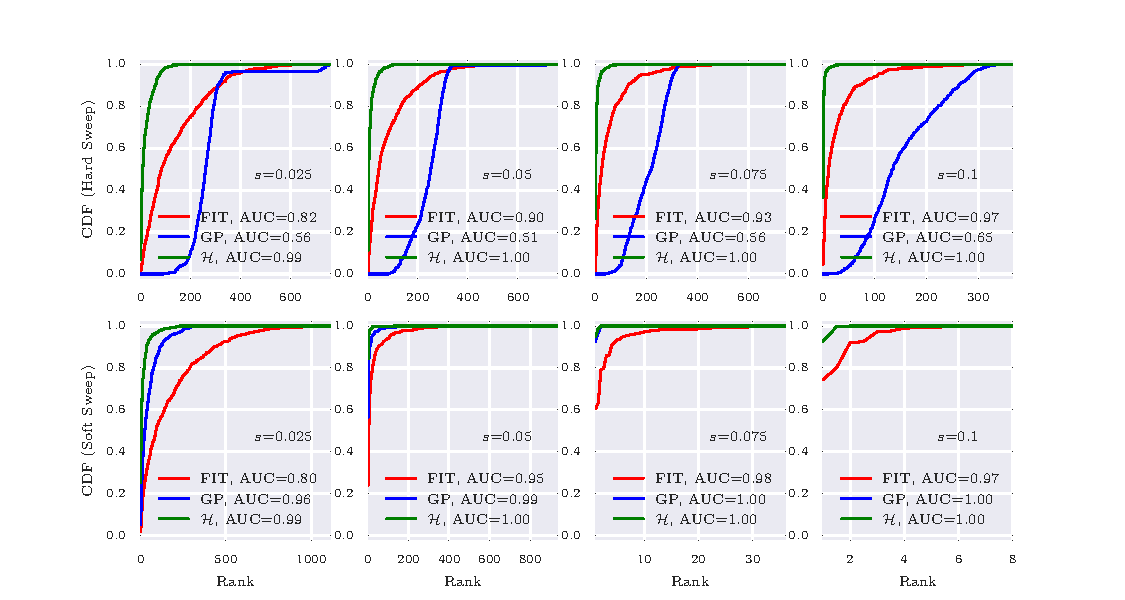
\includegraphics[trim=.2in 0 .2in 0, 
	clip,width=\textwidth]{figures/rankinf.pdf}
	\caption{Cumulative Distribution  Function (CDF) of the distribution of the 
	rank of the adaptive allele in 500 simulations for Markov Chain ($\Mc$), 
	Gaussian Process (GP) and Frequency Increment Test (FIT), for different 
	values of selection strength $s$ and initial carrier frequency. Area Under 
	Curve (AUC) is computed as a quantitative measure ranking performance of 
	methods for each configuration.}
	\label{fig:rankinf}
\end{figure}
\end{document}
